% !TeX spellcheck = en-US
% !TeX encoding = utf8
% !TeX program = pdflatex
% !BIB program = biber
% -*- coding:utf-8 mod:LaTeX -*-


% vv  scroll down to line 200 for content  vv


\let\ifdeutsch\iffalse
\let\ifenglisch\iftrue
\input{pre-documentclass}
\documentclass[
  % fontsize=11pt is the standard
  a4paper,  % Standard format - only KOMAScript uses paper=a4 - https://tex.stackexchange.com/a/61044/9075
  twoside,  % we are optimizing for both screen and two-side printing. So the page numbers will jump, but the content is configured to stay in the middle (by using the geometry package)
  bibliography=totoc,
  %               idxtotoc,   %Index ins Inhaltsverzeichnis
  %               liststotoc, %List of X ins Inhaltsverzeichnis, mit liststotocnumbered werden die Abbildungsverzeichnisse nummeriert
  headsepline,
  cleardoublepage=empty,
  parskip=half,
  %               draft    % um zu sehen, wo noch nachgebessert werden muss - wichtig, da Bindungskorrektur mit drin
  draft=false
]{scrbook}
\input{config}


\usepackage[
  title={A Tool for the Estimation of Lattice Parameters},
  author={Nicolai Krebs},
  type=bachelor,
  institute=sec, % or other institute names - or just a plain string using {Demo\\Demo...}
  course={Informatik, B.Sc.},
  examiner={Prof.\ Dr.\ Ralf Küsters},
  supervisor={Marc Rivinius,\ M.Sc.},
  startdate={April 22, 2021},
  enddate={October 22, 2021}
]{scientific-thesis-cover}

\input{acronyms}

\makeindex

\begin{document}

%tex4ht-Konvertierung verschönern
\iftex4ht
  % tell tex4ht to create picures also for formulas starting with '$'
  % WARNING: a tex4ht run now takes forever!
  %\Configure{$}{\PicMath}{\EndPicMath}{}
  %$ % <- syntax highlighting fix for emacs
  \Css{body {text-align:justify;}}

  %conversion of .pdf to .png
  \Configure{graphics*}
  {pdf}
  {\Needs{"convert \csname Gin@base\endcsname.pdf
      \csname Gin@base\endcsname.png"}%
    \Picture[pict]{\csname Gin@base\endcsname.png}%
  }
\fi

%\VerbatimFootnotes %verbatim text in Fußnoten erlauben. Geht normalerweise nicht.

\input{commands}
\pagenumbering{arabic}
\Titelblatt

%Eigener Seitenstil fuer die Kurzfassung und das Inhaltsverzeichnis
\deftriplepagestyle{preamble}{}{}{}{}{}{\pagemark}
%Doku zu deftriplepagestyle: scrguide.pdf
\pagestyle{preamble}
\renewcommand*{\chapterpagestyle}{preamble}



%Kurzfassung / abstract
%auch im Stil vom Inhaltsverzeichnis
\ifdeutsch
  \section*{Kurzfassung}
\else
  \section*{Abstract}
\fi

<Short summary of the thesis>

\cleardoublepage


% BEGIN: Verzeichnisse

\iftex4ht
\else
  \microtypesetup{protrusion=false}
\fi

%%%
% Literaturverzeichnis ins TOC mit aufnehmen, aber nur wenn nichts anderes mehr hilft!
% \addcontentsline{toc}{chapter}{Literaturverzeichnis}
%
% oder zB
%\addcontentsline{toc}{section}{Abkürzungsverzeichnis}
%
%%%

%Produce table of contents
%
%In case you have trouble with headings reaching into the page numbers, enable the following three lines.
%Hint by http://golatex.de/inhaltsverzeichnis-schreibt-ueber-rand-t3106.html
%
%\makeatletter
%\renewcommand{\@pnumwidth}{2em}
%\makeatother
%
\tableofcontents

% Bei einem ungünstigen Seitenumbruch im Inhaltsverzeichnis, kann dieser mit
% \addtocontents{toc}{\protect\newpage}
% an der passenden Stelle im Fließtext erzwungen werden.

\listoffigures
\listoftables

%Wird nur bei Verwendung von der lstlisting-Umgebung mit dem "caption"-Parameter benoetigt
%\lstlistoflistings
%ansonsten:
\ifdeutsch
  \listof{Listing}{Verzeichnis der Listings}
\else
  \listof{Listing}{List of Listings}
\fi

%mittels \newfloat wurde die Algorithmus-Gleitumgebung definiert.
%Mit folgendem Befehl werden alle floats dieses Typs ausgegeben
\ifdeutsch
  \listof{Algorithmus}{Verzeichnis der Algorithmen}
\else
  \listof{Algorithmus}{List of Algorithms}
\fi
%\listofalgorithms %Ist nur für Algorithmen, die mittels \begin{algorithm} umschlossen werden, nötig

% Abkürzungsverzeichnis
\printnoidxglossaries

\iftex4ht
\else
  %Optischen Randausgleich und Grauwertkorrektur wieder aktivieren
  \microtypesetup{protrusion=true}
\fi

% END: Verzeichnisse


% Headline and footline
\renewcommand*{\chapterpagestyle}{scrplain}
\pagestyle{scrheadings}
\pagestyle{scrheadings}
\ihead[]{}
\chead[]{}
\ohead[]{\headmark}
\cfoot[]{}
\ofoot[\usekomafont{pagenumber}\thepage]{\usekomafont{pagenumber}\thepage}
\ifoot[]{}


%% vv  scroll down for content  vv %%































%%%%%%%%%%%%%%%%%%%%%%%%%%%%%%%%%%%%%%%%%%%%%%%%%%%%%%%%%%%%%%%%%%%%%%%%%%%%%%
%
% Main content starts here
%
%%%%%%%%%%%%%%%%%%%%%%%%%%%%%%%%%%%%%%%%%%%%%%%%%%%%%%%%%%%%%%%%%%%%%%%%%%%%%%


\chapter{Introduction}\label{sec:intro}

- rise of quantum computing (short history)

* conceptual

* reality


- problem: some hard classical problems no longer hard

* Shor's Algorithm (Peter Shor, 1994) %Sho97
=> quantum computers can solve the factoring and the discrete logarithm problem in polynomial time

* application to encryption

* overview of current encryption methods that will become insecure


- one solution (among hash-based, code-based, isogeny-based, and multivariate): lattice crypto

* overview over history and capability of lattice crypto

* advantages: good (quasilinear) asymptotic key sized, good concrete runtimes and key sizes, worst-case secure instantiations, advanced cryptographic primitives previously infeasible

* including intro to LWE/SIS and applications to build crypto systems

. SIS: signature schemes, hash functions

. LWE: ``cryptomania'' applications (PKE, ...), signature schemes, lines:
% TODO: more content in comment under lattice background

- cryptographic applications

- establishing theoretical and asymptotic hardness \cite{Reg05} % ? Check
\cite{BLPRS13, MP13}
- concrete hardness of LWE: attacks, runtime estimates,

* briefly outline concept and benefits of hard-case to average-case reductions


- purpose of this thesis

* building schemes: need realistic hardness estimates of schemes for given parameter settings

* lack in the past: no unified/easy to use tool => thesis aims to solve this problem
tool we call \textit{Lattice Parameter Estimation} % TODO: too long. Maybe just "tool"?
LWE instances are estimated by calling various estimation functions from the LWE Estimator \cite{APS15}, which we will refer to as \textit{estimator}.


- overview of chapters/how to read



\chapter{Preliminaries} \label{chap:Preliminaries}
% short summary/

% TODO: check out MG02 for more details for this section!!!

% TODO: some algebraic background

\section{Notation}
In the following, we denote vectors by bold lower-case letters like $\mathbf{v}$ and matrices by bold upper-case letters $\mathbf{M}$. We interchangably use matrix notation and sets of column vectors $\left[\mathbf{v}_1 \cdots \mathbf{v}_n\right] = \left\{\mathbf{v}_1, \dots, \mathbf{v}_n\right\}$. Unless specified otherwise, by $\| \cdot \|$ or simply \textit{norm} we refer to the Euclidean norm. By $[n]$ we denote the set $\{1, \dots, n\}$ for $n\in \mathbb{Z}^+$.
% TODO: anything else? Inner product, negation in ring

\section{Norms}\label{sec:norms}
We can define the standard $\ell_p$-norms on the vector space $\mathbb{R}^n$. In this work we will also consider rings and modules (see \cref{sec:ring-module}) and require a way to bound the length of ring and module elements. Let $\mathcal{R}_q=\mathbf{Z}_q[X]/\langle X^n + 1 \rangle$ be a quotient ring as defined in \cite{BDLOP18} and $f \in \mathcal{R}_q$ with $f = \sum_i f_i X^i$. Following \cite{BDLOP18} we define the norms
\begin{equation}
    \begin{aligned}
        \ell_1 : \| f \|_1           & = \sum_i |f_i|,                                         \\
        \ell_2 : \| f \|_2           & = \sqrt{\sum_i |f_i|^2} \text{ and}                     \\
        \ell_p : \| f \|_p           & = \left(\sum_i |f_i|^p\right)^{\frac{1}{p}} \text{ and} \\
        \ell_\infty : \| f \|_\infty & = \max_i |f_i|.
    \end{aligned}
\end{equation}
For standard vector spaces, the definitions are essentially equivalent to the above, except that $f$ is a vector in $\mathbb{R}^n$ with coefficients $f_i$. For a module element $\mathbf{f} \in \mathcal{R}_q^d$, we can simply view $\mathbf{f}$ as a $n\cdot d$-dimensional vector.

\section{Lattices}
%%%%%%%%%%%%%%%%%%%%%%%%%%%%%%%%%%%%%%%%%%%%%%%%%%%
% maybe put in intro
Lattices have been used in cryptography since the end of the last century. Lattice reduction algorithms such as the LLL algorithm resulted in a number of practical attacks on popular cryptosystems \cite{NV10}. The landmark work of Ajtai \cite{Ajt96} opened up the way for a new family of cryptosystems. He showed that any instance of a certain lattice problem, the approximate Shortest Vector Problem (SVP$_\gamma$) can be reduced to a randomized instance of the Short Integer Solution (SIS) problem. In particular, this implies that an average-case SIS instance is at least as hard as a worst-case instance of SVP$_\gamma$, resulting in extremely strong security guarantees. Later, Regev came up with a similar worst-case to average-case reduction for the Learning with Errors (LWE) problem \cite{Reg05}.

% TODO: the following could be move to intro
% * fully homomorphic [Gen09]

% * BGV scheme [BV11, BGV12]

% * tools [LPR10, LPR13] ideal latties, RLWE

% Other Notes: %TODO
% - PKE \cite{AD97, Reg03, Reg05}, CCA security \cite{PW08, Pei09}, identity-based encryption \cite{GPV08, CHKP10, ABB10}, fully homomorphic \cite{Gen09a}
% - , LWE introduced by \cite{Reg05} "provably as hard as certain lattice problems in worst case, appear to require time exponential in main security parameter to solve"
% - NTRU \cite{HPS98}
% - $q$-ary lattice: modulus $q\geq 2$

% Applications: SIS can be used for one-way functions and collision-resistant hasing. LWE can be used to build pseudo-random number generators, public-key encryption schemes and oblivious transfer and secure MPC. Lattice Trapdoors (trapdoor functions, digital signatures)? Punctured Trapdoors (identity-based encryption, attribute-based encryption, predicate encryption)? % TODO: from https://www.youtube.com/watch?v=LlPXfy6bKIY see below for more detail

% % TODO: move to intro 
% % - introduced in \cite{MR04}, origins in \cite{Ajt96}, used for ´minicrypt´ primitives: one-way functions \cite{Ajt96}, collision resistant hash functions \cite{GGH96}, digital signature schemes \cite{GPV08, CHKP10}, and identification schemes \cite{MV03, Lyu08, KTX07} % TODO change or \cite{Reg10}

% Following based on \cite{Reg10}:% TODO: change or quote 

% Introduced by Regev in \cite{Reg09}
% Origin: work of Ajtai and Dwork \cite{AD97}, first public-key cryptosystem based on worst-case lattice problems, simlifications/improvements \cite{GGH97b, Reg03} imply hardness result for LWE.
% Early work: hardness based on unique-SVP, Peikert \cite{Pei09} and Lyubashevsky and Micciancio \cite{LM09} show that unique-SVP is essentially equivalent to \textsc{GapSVP}.

% - ´cryptomania´ applications: public-key encryption schemes under chosen-plaintext attacks \cite{Reg05, KTX07, PVW08}, and chosen-ciphertext attacks \cite{PW08, Pei09}, oblivious transfer protocoles \cite{PVW08}, identity-based encryption (IBE) schemes \cite{GPV08, CHKP10, ABB10}, leakage-resilient encryption \cite{AGV09, ACPS09, DGKPV10, GKPV10}, and more % TODO change or \cite{Reg10}

% - most important: fully homomorphic encryption schemes \cite{Gen09a, BV11, Bra12, GSW13} % TODO 
%%%%%%%%%%%%%%%%%%%%%%%%%%%%%%%%%%%%%%%%%%%%%

We now present the mathematical definition of lattices and related tools that we will use later on. Most of the background theory is based on material from \cite{MG02} with some adaptions.

A \textit{lattice} $\Lambda$ is a discrete additive subgroub of the vector space $\mathbb{R}^m$. Every lattice can be defined by a basis $\mathbf{B}$ of $n$ linearly independent basis vectors $\mathbf{b}_1, \ldots, \mathbf{b}_n \in \mathbb{R}^m$ with $m\geq n$. A lattice then is the set of all integer linear combinations of the basis vectors in $\mathbf{B}$.

\begin{definition}[Lattice]
    Given a basis $\mathbf{B} = \left[\mathbf{b}_1, \ldots, \mathbf{b}_n\right] \in \mathbb{R}^{m\times n}$. We call $\Lambda$ a lattice generated by the column vectors of $\mathbf{B}$ if
    \begin{equation}
        \Lambda(\mathbf{B}) = \left\{ \mathbf{x} \in \mathbb{R}^m \;\middle\vert\ \; \exists c_1, \ldots, c_n \in \mathbb{Z} : \mathbf{x} = \sum_{i=1}^n c_i \mathbf{b}_i \right\}.
    \end{equation}
\end{definition}

% TODO: make plot
We call $n$ the \textit{rank} of the lattice. A lattice has full rank if the $n=m$. The basis of a lattice $\mathbf{B}$ is not unique. If $\mathbf{B}$ is a basis of a lattice $\Lambda$ then for any unimodular matrix $\mathbf{U}\in \mathbb{Z}^{n\times n}$ with determinant $\pm 1$ the basis $\mathbf{B}\cdot \mathbf{U}$ is also a basis of $\Lambda$. In cryptographic applications, we usually start with a lattice basis $\mathbf{B}$ with long basis vectors that are not very orthogonal to each other. For example, the problem of finding a short vector (SVP or SVP$_\gamma$, see \cref{def:svp}) in $\Lambda(B)$ turns out to be very difficult. If we can somehow find a ``nicer'' basis for $\Lambda(B)$ with shorter and more orthogonal basis vectors, finding a solution becomes a lot easier. We can improve the quality of a basis or ``reduce'' a basis in such a way by means of lattice basis reduction. But more to that later.
% TODO example plot

% TODO: do we need cosets???

Similar to a quotient ring $\mathbb{Z}/q\mathbb{Z}$ of integers modulo some positive integer $q$ with cosets $c + q\mathbb{Z}$, we can define the quotient group $\mathbb{R}^m/\mathbf{\Lambda}$ with \textit{cosets}
\begin{equation}
    \mathbf{c} + \Lambda = \{\mathbf{c} + \mathbf{v} \mid \mathbf{v}\in \Lambda\}
\end{equation}
where $\mathbf{c} \in \mathbb{R}^m$ \cite{Pei16}. % TODO: maybe add plot

An important concept is the \textit{fundamental domain} of a lattice. The fundamental domain is a subset of $\mathbb{R}^m$ that contains exactly one representative of every coset of $\mathbb{R}^m/\mathbf{\Lambda}$. The most commonly considered fundamental domain of a lattice with basis $\mathbf{B}$ is the (shifted) \textit{fundamental parallelipiped}
\begin{equation} \label{eq:fundamental-parallelipiped}
    \mathcal{P}_{\frac{1}{2}}(\mathbf{B}) = \mathbf{B} \cdot \left[ - \frac{1}{2}, \frac{1}{2}\right)^n = \left\{ \mathbf{x} \in \mathbb{R}^m \;\middle|\; \mathbf{x} = \sum_{i=1}^n c_i \mathbf{b}_i, \; c_i \in  \left[ - \frac{1}{2}, \frac{1}{2}\right) \right\}
\end{equation}
Another region that is often used is the \textit{Voronoi region} $\mathcal{V}$ \cite{GJS15} and is defined as
\begin{equation}\label{eq:voronoi-region}
    \mathcal{V} = \left\{ \mathbf{x} \in \mathbb{R}^n \mid \forall \mathbf{y} \in \Lambda : \| \mathbf{x} \| \leq \| \mathbf{x} - \mathbf{y} \| \right\}.
\end{equation}
% every coset has representative  % c - B * \left\lfloor^{-1} \cdot c\right\rceil
% TODO: first define [0, 1)
% intuition: collection of all points that can be written as By where y in [0, 1)^n
% TODO: maybe add plot

The $n$-dimensional volume of the fundamental parallelipiped of a lattice $\Lambda(\mathbf{B})$ is equivalent to the \textit{determinant} of the lattice $\text{det}(\Lambda(\mathbf{B})) = \sqrt{\text{det}\left(\mathbf{B}^\intercal \mathbf{B}\right)}$. For a full-ranked lattice the determinant becomes $\det(\Lambda(\mathbf{B})) = |\det(\mathbf{B})|$. The determinant is independent from the used basis which can be easily verified by considering  $\text{det}(\Lambda(\mathbf{U}\mathbf{B})$.

The \textit{minimum distance} $\lambda_1(\Lambda)$ of a lattice is the length of its shortest nonzero vector
\begin{equation}
    \lambda_1(\Lambda) = \min_{v \in \Lambda \setminus \{0\}}\|\mathbf{v}\|.
\end{equation}
Furthermore, we can define \textit{$i$th successive minima} $\lambda_i(\Lambda)$ by considering an $m$-dimensional ball $\mathcal{B}(\mathbf{0}, r)$ with increasing radius $r \in \mathbb{R}$ and center $\mathbf{0} \in \mathbb{R}^m$ at the origin of $\Lambda$. Then  $\lambda_i(\Lambda)$ is the smallest radius $r$ such that the ball $\mathcal{B}(\mathbf{0}, r)$ contains exactly $i$ linearly independent lattice vectors. Note that an optimally reduced basis with basis vectors $\mathbf{b}_1 \leq \mathbf{b}_2 \cdots \leq \mathbf{b}_n$ satisfies $\lambda_i(\Lambda) = \|mathbf{b}_i\|$ for all $i\in [n]$.


In general it is hard to determine the exact values of $\lambda_i(\Lambda(\mathbf{B}))$ for a given basis $\mathbf{B}$. \textit{Minkowski theorem} states that $\lambda_1(\Lambda) \leq \sqrt{n} \cdot (\det(\Lambda))^{\frac{1}{n}}$ given that $\Lambda$ has rank $n$.
The \textit{Gaussian heuristic} is commonly used to estimate the minimum distance $\lambda_1$ of a lattice $\Lambda$ given the determinant $\det{\Lambda}$:
\begin{equation}\label{eq:gaussian-heuristic}
    \lambda_1(\Lambda) \approx \frac{\Gamma(1 + n/2)^{1/n}}{\sqrt{\pi}} \det(\Lambda)^{1/n}
\end{equation}
By applying Stirling's formula to estimate the $\Gamma$-function as described in \cite{Gop16}, we can simply the estimate to
\begin{equation}\label{eq:simplified-gaussian-heuristic}
    \lambda_1(\Lambda) \approx \sqrt{\frac{n}{2\pi e}} \det(\Lambda)^{1/n}
\end{equation}

% TODO: dual lattice
The dual $\Lambda^{\perp}$ of a lattice $\Lambda(\mathbf{B})$ is defined as the set of vectors $\mathbf{y}$ in the span of $\mathbf{B}$ such that the inner product $\langle \mathbf{y}, \mathbf{v} \rangle$  is an integer for all $\mathbf{v} \in \Lambda(\mathbf{B})$. The basis the dual of a lattice with basis $\mathbf{B}$ is given by $\mathbf{B'} = \mathbf{B} (\mathbf{B}^\intercal \mathbf{B})^{-1}$.

In cryptography, we are mainly interested in modular integer (or $q$-ary) lattices. A $q$-ary lattice is a lattice $\Lambda_q$ such that $q\mathbb{Z}^m \subseteq	\Lambda \subseteq	\mathbb{Z}^m$ given $q \in \mathbb{N}\setminus \{0\}$. This means that a vector $\mathbf{x} \in \mathbb{Z}^m$ is in $\Lambda$ if and only if $\mathbf{x} \mod q$ also is in $\Lambda$.

We now look at two important ways of specifying a $q$-ary lattice given a matrix $\mathbf{A} \in \mathbb{Z}_q^{n\times m}$ \cite{BBGS19}.\begin{equation}\label{eq:lwe-lattice}
    \Lambda_q(\mathbf{A}^\intercal) = \left\{ \mathbf{v} \in \mathbb{Z}^m \mid \exists \mathbf{y} \in \mathbb{Z}^n : \mathbf{v} = \mathbf{A}^\intercal \mathbf{y} \mod q \right\}
\end{equation}
$\Lambda_q(\mathbf{A}^\intercal)$ is commonly referred to as the \textit{(primal) LWE lattice} as finding a short vector in $\Lambda_q(\mathbf{A}^\intercal)$ corresponds to solving LWE. The second, referred to as the \textit{(dual) SIS lattice}, is given by
\begin{equation}\label{eq:sis-lattice}
    \Lambda_q^\perp(\mathbf{A}) = \left\{ \mathbf{v} \in \mathbb{Z}^m \mid  \mathbf{A}\mathbf{v} = \mathbf{0} \mod q \right\}.
\end{equation}
Finding a short vector in $\Lambda_q^\perp(\mathbf{A})$ corresponds to solving the Short Integer Solution problem.

% TODO: find basis of $\Lambda_q(\mathbf{A})$ \cite{AFG13}

In many scenarios, it is convenient to have an explicit formula that descibes the relationship between the determinant of the above two lattices and the dimensions of $\mathbf{A}$. For $q$ prime and $m$ sufficiently larger than $n$ we have that the rank of $\mathbf{A}$ is $n$ as the rows of $\mathbf{A}$ are linearly independent with high probability. As a result, the lattice $\Lambda_q(\mathbf{A}^\intercal)$ has $q^n$ points in $\mathbb{Z}_q^m$.
Consider the fundamental domain $D = \mathcal{P}(\Lambda_q(\mathbf{A}^\intercal))$ and the fact that $\Lambda_q(\mathbf{A}^\intercal) + (D \mod q) = \mathbb{R}^m/q\mathbb{R}^m$ is a partition as described in \cite{volume-lattice}. The volume of $\mathbb{R}^m/q\mathbb{R}^m$ is given by $q^m =|\Lambda_q(\mathbf{A}^\intercal)||D \mod q|$ and thus
\begin{equation}\label{eq:det-MR}
    \text{det}(\Lambda_q(\mathbf{A}^\intercal)) = |D \mod q| = \frac{q^m}{|\Lambda_q(\mathbf{A}^\intercal)|} = \frac{q^{m}}{q^{n}} = q^{m-n}.
\end{equation}
Furthermore, we know that the dual lattice  $\Lambda_q^\perp(\mathbf{A})$ has $q^{m-n}$ points in $\mathbb{Z}_q^m$ as the dimension of the kernel of $\mathbf{A}$ is $m-n$. Analogously, we obtain
\begin{equation}\label{eq:det-MR-dual}
    \text{det}(\Lambda_q(\mathbf{A}^\intercal)^{\perp}) = |D \mod q| = \frac{q^m}{|\Lambda_q(\mathbf{A}^\intercal)^{\perp}|} = \frac{q^{m}}{q^{m-n}} = q^n.
\end{equation}


Another useful tool it the \textit{Gram-Schmidt orthogonalization} \label{sec:gram-schmidt}. Given a basis $\mathbf{B} = \left[\mathbf{b}_1 \cdots \mathbf{b}_n\right] \in \mathbb{Z}_q^{m\times n}$, we write $\pi_{\text{span}(\mathbf{B})}(\mathbf{t})$ for projection of a vector $\mathbf{t}$ onto the span of the vectors in $\mathbf{B}$.
% or, more formally,
% \begin{equation}
%   \pi_{\text{span}(\mathbf{B})}(\mathbf{t}) = \mathbf{B}(\mathbf{B}^\perp \mathbf{B})^{-1}\mathbf{B}^\intercal \cdot \mathbf{t}
% \end{equation}
Define $\tilde{\mathbf{b}}_i$ as follows: $\tilde{\mathbf{b}}_1 = \mathbf{b}_1$. For $i \in \{2, \ldots, n\}$ let $\tilde{\mathbf{b}}_i$ be the component of $\mathbf{b}_i$ that is orthogonal to the span of $\left\{\mathbf{b}_1, \ldots, \mathbf{b}_{i-1}\right\}$. In other words,
\begin{equation}
    \tilde{\mathbf{b}}_i = \mathbf{b}_i - \pi_{\text{span}(\mathbf{b}_1, \ldots, \mathbf{b}_{i-1})}(\mathbf{b}_i).
\end{equation} % TODO: define span?
Then,  $\tilde{\mathbf{B}} = \left[\tilde{\mathbf{b}}_1 \cdots \tilde{\mathbf{b}}_n\right]$ is called the Gram-Schmidt orthogonalization of the basis $\mathbf{B}$. We define the Gram-schmidt coefficients as follows:
\begin{equation}
    \mu_{i, j} = \frac{\left\langle \tilde{\mathbf{b}}_j, \mathbf{b}_i\right\rangle}{\left\langle \tilde{\mathbf{b}}_j, \tilde{\mathbf{b}}_j\right\rangle}
\end{equation}

% TODO Also check out algorithm from AGVW17

We define $\text{dist}(\mathbf{t}, \Lambda(\mathbf{B}))$ where $\Lambda(\mathbf{B}) \subset \mathbb{R}^m$ as the \textit{distance} of a vector $\mathbf{t} \in \mathbb{R}^m$ to the closest lattice vector $\mathbf{v} \in \Lambda(\mathbf{B})$, i.e., $\text{dist}(\mathbf{t}, \Lambda(\mathbf{B})) = \min_{\mathbf{v} \in \Lambda(\mathbf{B})}\|\mathbf{t} -  \mathbf{v}\|$.



% * smoothing lemma



\subsection{Lattice Problems}\label{sec:lattice-problems}
In the previous section, we already mentioned the Shortest Vector Problem or short SVP. In this section, we want to briefly list a number of lattice problems used in this work.

\begin{definition}[SVP$_\gamma$] \label{def:svp}
    Given a basis $\mathbf{B}$ of a lattice $\Lambda$, the (approximate) Shortest Vector Problem (SVP$_\gamma$) is the problem of finding a short lattice vector $v\in \Lambda$ such that $0 < \| v \| \leq \gamma \lambda_1(\Lambda)$.
\end{definition}

The corresponding decision version is the \textsc{GapSVP}$_\gamma$ problem in which we are asked to decide whether $\lambda_1(\Lambda) \leq 1$ or $\lambda_1(\Lambda) \geq \gamma$ given a basis $\mathbf{B}$ of $\Lambda$. If neither is the case, any answer is accepted. In an alternative version of \textsc{GapSVP}$_\gamma$ we have to decide between $\lambda_1(\Lambda) \leq d$ and $\lambda_1(\Lambda) \geq \gamma d$ for some positive real number $d$ \cite{LM09}.

\begin{definition}[SIVP$_\gamma$] \label{def:sivp}
    Given a basis $\mathbf{B}$ of a lattice $\Lambda$ of rank $n$, the (approximate) Shortest Independent Vector Problem (SIVP) is the problem of finding $n$ linearly independent lattice vectors $\mathbf{v}_1, \ldots, \mathbf{v}_n \in \Lambda$ such that $\|\mathbf{v}_i\| \leq \gamma \cdot \lambda_n(\Lambda)$ for all $i \in \{1, \ldots, n\}$.
\end{definition}

Both \textsc{GapSVP}$_\gamma$ and \textsc{SIVP}$_\gamma$ are NP-hard for any constant approximation factor $\gamma$ \cite{Khot05,BS99}. % in all $\ell_p$-norms 
% NP hard for any constant $\gamma$ % Kho04, HR07 see LM09
% fastest algorithm for $1\leq \gamma \leq \text{poly}(n)$ has runtime complexity of $2^{O(n)}$
In \cref{ch:algorithms}, we will look at some selected algorithms that rely on reductions to the following problems.

% \begin{definition}[CVP$_\gamma$] \label{def:gamma-CVP}
%   Given a basis $\mathbf{B}$ of a lattice $\Lambda \subset \mathbb{R}^m$ and a target vector $\mathbf{t}\in\mathbb{R}^m$, the (approximate)  Closest Vector Problem (CVP$_\gamma$) is the problem of finding a lattice vector $\mathbf{v} \in \Lambda$ with $\|\mathbf{t} - \mathbf{v}\| < \gamma \min_{\mathbf{v}' \in \Lambda} \|\mathbf{v}' - \mathbf{v}\|$.
% \end{definition}
% NP hard in any $\ell_p$-norm for approximation factor $\gamma=1$ \cite{vEB81}


% TODO: add some kind of discussion, e.g. see 1.2 in LM09 or better overview from bootcamp

% * ideal lattice (do I need that?)

% * ...?

% * eher die Sachen für LWE/SIS als die Sachen für Algorithmen (analog Vorlesung), evtl.

% Intuition für die anderen Sachen...



\section{Discrete Gaussian Distribution}

% - Gaussian, def, component-wise, trafo to bound % TODO: GPV08, or LS15

% * definition:
Oftentimes in lattice cryptography, we work with samples or vectors drawn from a discrete uniform or Gaussian distribution. We can define a discrete Gaussian distribution as follows:
\begin{definition}[Discrete Gaussian Distribution \cite{GJS15}]
    The discrete Gaussian distribution $D_{\Lambda, s, \mathbf{c}}$ over an $m$-dimensional lattice $\Lambda$ with width parameter $s > 0$ and center $\mathbf{c}$ is the probability distribution we obtain by assigning each vector $\mathbf{x}\in \Lambda$ a probability proportional to $e^{-\pi \|\mathbf{x} - \mathbf{c}\|^2/s^2}$. If $\mathbf{c} = \mathbf{0}$ we simply write  $D_{\Lambda, s}$.
\end{definition}
A discrete Gaussian sampler over a lattice can be efficiently realized (see for example \cite{GPV08}). In order to avoid confusion, throughout this work we use $\sigma$ to denote the standard deviation, where $\sigma = \frac{s}{\sqrt{2 \pi}}$, and define $\alpha = \frac{s}{q} = \frac{\sqrt{2\pi} \sigma}{q}$.

% * better definition in GPV08 => different definition needed for LWE??? % TODO
% * how to do this? => variant of Babai's ``nearest-plane'' algorithm, see \cite{GPV08} % TODO

% * component-wise

% * smoothing factor here?






\section{LWE and SIS}\label{sec:problems}
In \cref{sec:intro} we informally introduced the Learning with Errors (LWE) problem and the Short Integer Solution (SIS) problem that constitute the main focus of this work. Both problems have given rise to a great variety of cryptosystems, in particular, in the context of the imminent advent of quantum computing. Hence, their importance in modern cryptography cannot be understated. We will now continue to describe them in more detail.

\subsection{Learning with Errors (LWE)} \label{sec:lwe}
The \textit{Learning with Errors} (LWE) problem asks us to recover some secret vector $\mathbf{s} \in \mathbb{Z}_q^n$ from a sequence of perturbed random linear equations on $\mathbf{s}$. The perturbed linear equations, also called samples, are of form $\langle\mathbf{a}_i, \mathbf{s}\rangle + e_i \mod q$, where $\mathbf{a}_i \in \mathbb{Z}_q^n$ are $e_i$ are an error term. We obtain a total of $m$ samples and can thus also express the equation system that is to be solved as $\mathbf{z} = \mathcal{A}^\intercal \mathbf{s} + \mathbf{e} \mod q$, where $\mathcal{A} \in \mathbb{Z}^{n \times m}$ and $\mathbf{e} \in \mathbb{Z}^m$. Note that we only know $\mathbf{z}$ and $\mathbf{A}$. A formal definition follows.

\begin{definition}[LWE Distribution \cite{Reg10}] %TODO
    Given an integer $n \geq 1$, a modulus $q \geq 2$, an error distribution $\chi$ on $\mathbb{Z}_q$, and a fixed secret vector $\mathbf{s}$, let $\mathcal{A}_{\mathbf{s}, \chi}$ be the probability distribution over $\mathbb{Z}_q^n \times \mathbb{Z}_q$ by choosing a vector $\mathbf{a}_i \in \mathbb{Z}_q^n$ uniformly at random, $e_i \in \mathbb{Z}_q$ according to $\chi$.  $\mathcal{A}_{\mathbf{s}, \chi}$ outputs pairs of
    \begin{equation}
        (\mathbf{a}_i, \langle \mathbf{a}_i, \mathbf{s} \rangle + e_i \mod q) \in \mathbb{Z}_q^n \times \mathbb{Z}_q.
    \end{equation}
\end{definition}

Additions are performed in $\mathbb{Z}_q$. In the case of $q=2$ the LWE problem corresponds to the \textit{Learning Parity with Noise} (LPN) problem. % TODO still needed with Search-LWE\ldots???
We distinguish between two versions of LWE.

% TODO: error distribution => gaussian, paramter alpha, define?
% TODO matrix Schreibweise vs nicht matrix schreibweise
% TODO Define Search/Decision LWE? 
\begin{definition}[Search-LWE$_{n, q, m, \chi}$] % \cite{LP11}
    The Search-LWE$_{n, q, m, \chi}$ asks for the recovery of the secret vector $\mathbf{s}$ given $m$ independent samples $(\mathbf{a}_i, z_i) \leftarrow \mathcal{A}_{\mathbf{s}, \chi}$ % TODO matrix
\end{definition}

\begin{definition}[Decision-LWE$_{n, q, m, \chi}$]
    Given $m$ samples, the Decision-LWE$_{n, q, m, \chi}$ asks to distinguish whether the samples were drawn from $\mathcal{A}_{\mathbf{s}, \chi}$ or from a uniform distribution on $\mathbb{Z}_q^n \times \mathbb{Z}_q$.
\end{definition}

Intuitively, Search-LWE is at least as hard as Decision-LWE as a solution to Search-LWE trivially solves Decision-LWE. The other direction, however, also holds true \cite{Reg09} for a prime modulus $q=\text{poly}(n)$. % TODO: explain
The equivalence of the search and decision versions is convenient when we consider common attacks against LWE, some of which solving Decision-LWE and other Search-LWE (see \cref{ch:algorithms}).

% TODO: 
% Mic02, PR06, LM06 Ring-SIS hardness - SIVP (GapSVP is easy on ideal lattices)
% 


% TODO: show more about decoding problem?
% TODO: Einheitsmatrix in notation
% TODO: notation \mathbf{x} = (x_1, \ldots, x_n) is column vector and  \mathbf{x}^\intercal its corresponding tranpose
% TODO: add somewhere we assume that m > n
\subsubsection{LWE as a Decoding Problem} \label{sec:lwe-decoding}
We request $m$ samples $(\mathbf{a}_1, z_1), \ldots, (\mathbf{a}_m, z_m)$ where $z_i = \langle \mathbf{a}_i, \mathbf{s} \rangle + e_i \in \mathbb{Z}_q$ and $\mathbf{s} \in \mathbb{Z}_q^n$. Let $A = \left[ \mathbf{a}_1 \cdots \mathbf{a}_m\right] \in \mathbb{Z}_q^{n\times m}$, $\mathbf{z} = \left[z_1, \ldots, z_m\right]^\intercal$ and $e = \left[e_1, \ldots, e_n\right]^\intercal \in \mathbb{Z}_q^n$. Hence, we can formulate LWE as a decoding problem as in \cite{GJS15}:
\begin{equation} \label{eq:lwe-decoding}
    \mathbf{z} =  \mathbf{A}^\intercal \mathbf{s} + \mathbf{e}
\end{equation}
with generator matrix $\mathbf{A}$ for a linear code over $\mathbb{Z}_q$ and $\mathbf{z}$ as the received word (see \cref{sec:linear-code} for more details about linear codes). Finding the secret vector $\mathbf{z}$ is equivalent to finding the codeword $\mathbf{y} = \mathbf{A}^\intercal\mathbf{s}$ with minimum distance $\| \mathbf{y} - \mathbf{z} \|$.

We can transform an LWE$_{n, q, m, \chi}$ instance with a secret vector $\mathbf{s}$ chosen according to a uniform distribution into an LWE$_{n, q, m-n, \chi}$ instance with a secret vector $\hat{\mathbf{s}}$ chosen according to the error distribution $\chi$ at a loss of $n$ samples as follows \cite{GJS15}: Let $\mathbf{A}_0 = \left[ \mathbf{a}_1 \cdots \mathbf{a}_n\right]$ where $\mathbf{a}_1, \ldots, \mathbf{a}_n$ are the first $n$ columns of $\mathbf{A}$. We introduce new variables $\hat{\mathbf{s}} = \mathbf{A}^\intercal_0 \mathbf{s}  - \left[z_1, \ldots, z_n\right]^\intercal = \left[e_0, \ldots, e_n\right]^\intercal$ and $\hat{\mathbf{A}} = \mathbf{A}_0^{-1} \mathbf{A} = \left[\mathbf{I} \; \hat{\mathbf{a}}_{n+1} \cdots \hat{\mathbf{a}}_{m}\right]$ and compute $\hat{\mathbf{z}} = \mathbf{z} -  \hat{\mathbf{A}}^\intercal \left[z_1, \ldots, z_n\right]^\intercal  = \left[\mathbf{0}, \hat{z}_{n+1} \cdots \hat{z}_{m} \right]^\intercal$. Our new LWE instance has samples $(\hat{\mathbf{a}}_{n+1}, \hat{z}_{n+1}), \dots, (\hat{\mathbf{a}}_{m}, \hat{z}_{m})$. \label{sec:lwe-transform-distro}
% TODO: where do we need that? maybe move there, cite somewhere \e.g. KF15, ACPS, BLPRS13 classical hardness of learning with errors

% TODO parameter choice: often prime q \in poly(n), \chi has mean zero and \sigma = \alpha \cdot q for some small \alpha, e.g. Regev: q \approx n^2, \alpha = 1/(\sqrt{2\pi n} \cdot \log_2^2 n)

\subsubsection{LWE as a BDD Problem} \label{sec:lwe-bdd} % \cite{LP11}
Solving LWE also corresponds to solving the \textit{Bounded Distance Decoding problem} (BDD) in the lattice $\Lambda(\mathbf{A}^\intercal) = \{ \mathbf{x} \in \mathbb{Z}_q^m \mid \exists \mathbf{s} \in \mathbb{Z}_q^n : \mathbf{x} = \mathbf{A}^\intercal \mathbf{s}  \mod q \}$, where the $m$ columns of $\mathbf{A}$ correspond to the vectors $\mathbf{a}_i \in \mathbb{Z}_q^n$ of $m$ independent LWE samples $(\mathbf{a}_i, z_i) \leftarrow \mathcal{A}_{\mathbf{s}, \chi}$ and the components $z_i$ correspond to a perturbed lattice point in $\Lambda(\mathbf{A}^\intercal)$. % TODO check ^\intercal


\subsubsection{Hardness} \label{sec:lwe-hardness}
% % TODO
% Best algorithm to solve LWE: Blum, Kalai, and Wasserman \cite{BKW03} with $2^{O(n)}$ samples and time. % TODO Sketch BKW?
The most important hardness results for LWE come from \cite{Reg05} and \cite{Pei09}. Regev showed that there exists a polynomial-time quantum reduction from worst-case \textsc{GapSVP}$_\gamma$ and SIVP$_\gamma$ in the $\ell_2$-norm to the (average-case) search version of LWE. That means that LWE is quantumly at least as hard as \textsc{GapSVP}$_\gamma$ and SIVP$_\gamma$. A similar classical probabilistic polynomial-time reduction from worst-case \textsc{GapSVP}$_\gamma$ was later proposed by Peikert for a sufficiently large modulus $q\geq 2^n$ in any $\ell_p$-norm for $p \geq 2$. The Shortest Vector Problem and its variants are well studied problems that are NP-hard for certain approximation problems (see \cref{sec:lattice-problems}. To this point, it is assumed that no efficient quantum algorithms exist that can solve NP-hard problems. It is thus conjectured that cryptosystems based on the worst-case to average-case reductions from Regev and Peikert are secure, even in the context of quantum computing. The currently best algorithms solve LWE in $2^{O(n)}$ time.




\subsection{Short Integer Solution (SIS)}
The dual problem to LWE is the \textit{Short Integer Solution problem} (SIS).
In SIS problem, we are given a set of uniformly random vectors $\mathbf{a}_1, \ldots, \mathbf{a}_m \in \mathbb{Z}_q^n$ and asked to find an integer linear combination with small coefficients that sums to zero the zero vector (modulo $q$). A formal definition follows. % TODO change or \cite{Reg10}

% TODO: move to intro 
% - introduced in \cite{MR04}, origins in \cite{Ajt96}, used for ´minicrypt´ primitives: one-way functions \cite{Ajt96}, collision resistant hash functions \cite{GGH96}, digital signature schemes \cite{GPV08, CHKP10}, and identification schemes \cite{MV03, Lyu08, KTX07} % TODO change or \cite{Reg10}

\begin{definition}[SIS Problem, adapted from \citealp{LS15}]
    The problem \text{SIS}$_{n, q, m, \beta}$ is defined as follows: Given a uniformly random matrix $\mathbf{A}^{n\times m}$, find a vector $\mathbf{s} \in \mathbb{Z}^m$ such that $\mathbf{A} \cdot \mathbf{s} = \mathbf{0} \mod q$ and $0 < \| \mathbf{s}\| \leq \beta$.
\end{definition}

Finding such a vector corresponds to solving SVP$_\gamma$ in the scaled $q$-ary dual lattice $\Lambda_q^\perp(\mathbf{A}) = \left\{ \mathbf{v} \in \mathbb{Z}^m \mid  \mathbf{A}\mathbf{v} = \mathbf{0} \mod q \right\}$. Note that the problem becomes trivial for sufficiently large bounds $\beta$. If $\beta\geq q$ in any $\ell_p$-norm we can simply choose $\mathbf{s} = [q, 0, \dots, 0]^\intercal$. In some scenarios, the vector $\mathbf{s}$ is restricted to $\mathbb{Z}_q^m$. However, depending on the used norm for the length of $\mathbf{s}$, we can still efficiently find $\mathbf{s}$ with $\|\mathbf{s}\|_p$ by using some standard linear equation solver $\|\mathbf{s}\|_p$, if $\{\mathbf{s}\in \mathbb{Z}_q^m \mid \|\mathbf{s}'\|_p \leq \beta\} = \mathbb{Z}_q^m$. For example, in the $\ell_\infty$-norm we have that $\beta=q$ is large enough. In \cref{sec:norm-bounds} we will define norm bound conversions to be able to express relationships between different  $\ell_p$-norms.

We obtain similar hardness results as for LWE. Micciancio and Regev show a reduction from SIVP$_\gamma$ in the worst-case to average-case SIS problem \cite{MR04}.
% Hardness: for any poly-bounded $m, \beta$ and for ``large enough'' prime $q$: SIS$_{n, q, m, \beta}$ is as hard as worst-case approx-SIVP (and \textsc{GapSVP}) to within $\beta \cdot \tilde{O}(\sqrt{n})$ factor

% TODO: application, perhaps something as in file:///C:/Users/Nico/OneDrive/Studium/Informatik/6BA/Supplemental%20Material/[BC%20Micciancio]%20The%20Short%20Integer%20Solutions%20Problem%20and%20Cryptographic%20Applications.pdf would be nice


\subsection{Ring and Module Variants}\label{sec:ring-module}
In practice, the base variants of LWE and SIS are not used due to large key sizes required for secure cryptoschemes. Consider the matrix $\mathbf{A} \in \mathbb{Z}_q^{m \times n}$. We usually require $m \in \Omega(n)$ which gives us at least a quadratic space complexity. We therefore want to decrease our key sizes. A way to do this is by using rings and modules as the underlying structure of LWE and SIS. Explaining the details regarding the ring and module variants of both problems would go beyond the scope of this work. Hence we will only provide a rough intuition following \cite{Reg10} and define the various problem variants of LWE and SIS. All of them are included in our tool.

Consider the following choice for $\mathbf{A}$ . We set $n=2^k$ for some $k > 0$ and choose the column vectors $\mathbf{a}$ of $\mathbf{A}$ in groups of size $n$. In each group we sample $\mathbf{a}_1 = [a_1, \ldots, a_n]^\intercal$ from the uniform distirbution over $\mathbb{Z}_q^{n}$. The remaining columns are rotations $\mathbf{a}_i = [a_i, \ldots, a_n, -a_1, \ldots, -a_{i-1}]^\intercal$ of the first vector in the group. Hence, a block of $n\times n$ only needs $O(n)$ memory reducing the size of $\mathbf{A}$ by a factor of $n$. In addition, it is possible to achieve speedups in the operations by means of the Fast Fourier Transformation.

In the ring variant, instead of vectors of the group $\mathbb{Z}_q^n$, the columns of $\mathbf{A}$ are chosen as elements of the ring $\mathbb{Z}_q\left[x\right] / \left\langle x^n + 1 \right\rangle$ which we call $\mathcal{R}_q$. We ensure that the  $x^n + 1$ is irreducible over the rationals by letting $n$ be a power of two. The disadvantage of powers of two is that our key size is rather coarse-grained which may result in a larger key size for a secure instance than needed up to a factor of two. Modules present themselves as a solution to this problem. Let $K=\mathbb{Q}(\theta)$ be a number field, where $\theta$ is an algebraic number with degree $n$, as defined in \cite{LS15}. A $\mathcal{R}$-module $\mathcal{M} \subseteq K^d$ with dimension or rank $d$ is a generalization of rings and vector spaces and is closed under addition and multiplication by elements of $\mathcal{R}$. We only consider the module $\mathcal{R}^d$ with ring dimension $n$ and module rank $d$. For more details on the mathematical background, please see \cite{LS15}. % TODO add more... define multiplication or ring elements, module elements?

% TODO: put norms here or refer to them...

\begin{definition}[RSIS \cite{LS15}]
    The Ring-SIS problem \text{RSIS}$_{n, q, m, \beta}$ is defined as follows: Given $a_1, \ldots, a_m \in \mathcal{R}_q$ chosen independently from the uniform distribution, find $s_1, \ldots, s_m \in \mathcal{R}$ such that $\sum_{i=1}^m \mathbf{a}_i \cdot s_i = 0 \mod q$ and $0 < \| \mathbf{s}\| \leq \beta$, where $\mathbf{s} = \left[s_1, \ldots, s_m\right]^\intercal \in \mathcal{R}^m$.
\end{definition} % TODO: need n? say sth more about n power of 2?
% TODO: matrix version?
We can interpret a ring element $r \in \mathcal{R}$ as an $n$ dimensional vector with coefficients $r_i$ such that $r = \sum_{i=0}^{n-1} r_i x^i$. If we compare RSIS to standard SIS, each $a_i$ in RSIS corresponds to a $n\times n$ block in the standard SIS matrix $\mathbf{A}$. The $n$ columns are obtained by rotation as described above. An RSIS$_{n, q, m, \beta}$ instance can thus be seen as an SIS$_{n, q, m \cdot n, \beta}$ instance.

\begin{definition}[MSIS \cite{LS15}]
    The Module-SIS problem \text{MSIS}$_{n, d, q, m, \beta}$ is defined as follows: Given  $\mathbf{a}_1, \ldots, \mathbf{a}_m \in \mathcal{R}_q^d$ chosen independently from the uniform distribution, find $s_1, \ldots, s_n \in \mathcal{R}$ such that $\sum_{i=1}^m a_i \cdot s_i = 0\mod q$ and $0 < \| \mathbf{s}\| \leq \beta$, where $\mathbf{s} = \left[s_1, \ldots, s_m\right]^\intercal \in \mathcal{R}^m$.
\end{definition} % TODO: need n? say sth more about n power of 2?
% TODO: matrix version?
As for RSIS, we can view the vectors $\mathbf{a}_i$ in MSIS as blocks of $\mathbf{A}$ in SIS. Each vector $\mathbf{a}_i$ has $d$ coefficients and corresponds to a $n\cdot d \times n$ block in $\mathbf{A}$. An MSIS$_{n, d, q, m, \beta}$ instance thus becomes an SIS$_{n\cdot d, q, m \cdot n, \beta}$ instance.

For LWE we will only list the definition of the ring and module variant. We are aware that we have not introduced the underlying math and refer the reader to \cite{LS15}. Let us just note here that $\mathcal{R}^\perp$ referes to the dual of $\mathcal{R}$.
\begin{definition}[Ring-LWE (RLWE) Distribution \cite{LS15}]
    Let $\chi$ be the error distribution distribution on $\mathbb{T}_{\mathcal{R}^\perp} = K_\mathbb{R} / \mathcal{R}^\perp$ and $s \in \mathcal{R}^\perp$ be the secret. Then we define $\mathcal{A}_{q, s, \chi}^{(\mathcal{R})}$ as the RLWE distribution on $\mathcal{R}_q \times \mathbb{T}_{\mathcal{R}^\perp}$ obtained by choosing $a \in \mathbb{R}_q$ uniformly at random and an error term $e \in \mathbb{T}_{\mathcal{R}^\perp}$ according to $\chi$, and returning samples $(a, (a \cdot s)/q + e)$.
\end{definition}

The search version of RLWE$_{n, q, m, \chi}$ asks us to find $s$ given $m$ samples from $\mathcal{A}_{q, s, \chi}^{(\mathcal{R})}$ with modulus $q\geq 2$ and $n$ the degree of the polynomial of $\mathcal{R}$. The decision version asks us to distinguish between $m$ samples from $\mathcal{A}_{q, s, \chi}^{(\mathcal{R})}$ and $m$ independent samples from the uniform distirbution over $\mathcal{R}_q \times \mathbb{T}_{\mathcal{R}^\perp}$.

\begin{definition}[Module-LWE (MLWE) Distribution \cite{LS15}]
    Let $\chi$ be the error distribution distribution on $\mathbb{T}_{\mathcal{R}^\perp}$ and $\mathbf{s} \in (\mathcal{R}^\perp)^d$ be the secret vector. Then we define $\mathcal{A}_{q, \mathbf{s}, \chi}^{(\mathcal{M})}$ as the MLWE distribution on $(\mathcal{R}_q)^d \times \mathbb{T}_{\mathcal{R}^\perp}$ obtained by choosing $\mathbf{a} \in (\mathbb{R}_q)^d$ uniformly at random and an error term $e \in \mathbb{T}_{\mathcal{R}^\perp}$ according to $\chi$, and returning samples $(\mathbf{a}, \frac{1}{q}\langle \mathbf{a},\mathbf{s}\rangle + e)$.
\end{definition}

Analogously, the search version of MLWE$_{n, d, q, m, \chi}$ asks us to find $\mathbf{s}$ given $m$ samples from $\mathcal{A}_{q, \mathbf{s}, \chi}^{(\mathcal{M})}$ with modulus $q\geq 2$, $n$ the degree of the polynomial of $\mathcal{R}$ and modulus rank $d$. The decision version asks us to distinguish between $m$ samples from $\mathcal{A}_{q, \mathbf{s}, \chi}^{(\mathcal{M})}$ and $m$ independent samples from the uniform distirbution over $\mathcal{R}_q^d \times \mathbb{T}_{\mathcal{R}^\perp}$.

We can construct a matrix $\mathbf{A}$ of the $a_i$ of RLWE and $\mathbf{a}_i$ of MLWE as for standard LWE to formulate the problems as a decoding problem as in \cref{sec:lwe-decoding} and interpret RLWE$_{n, q, m, \chi}$ and MLWE$_{n, d, q, m, \chi}$ as instances of LWE$_{n, q, m \cdot d, \chi'}$ and RLWE$_{n\cdot d, q, m \cdot n, \chi'}$ respectively.




% TODO: replace "hardness" with "complexity of solving"?
\chapter{Algorithms and Estimates}\label{ch:algorithms}
The main functionality of our tool relies on runtime cost estimation procedures for a number of popular algorithms that can be used to solve SIS or LWE. The estimates for LWE are provided by the $\textit{estimator}$ \cite{APS15}. In addition, we included cost estimates of two different approaches for SIS. Many of the algorithms we use rely on subprocedures, in particular lattice reduction algorithms, and there exist more realistic and more conservative estimates. Depending on the choice of attack algorithms and reduction cost models, the returned cost may differ significantly. Also, not all attack estimates perform well in practice. It is thus of interest to us to gain a basic understanding of how the respective algorithms work.


\section{Lattice Basis Reduction} % perhaps move to Algorithms
% For survey see Ngu11, NV10, MW16
In \cref{sec:problems} we showed how LWE and SIS can be viewed as lattice problems. % TODO: make sure all is there
However, the corresponding lattice basis that we obtain is rather ugly lattice basis with long basis vectors. Solving lattice problems in such a basis is infeasible. Our goal is thus to find a better basis with shorter and more orthogonal basis vectors. A family of algorithms that achieve just this is called lattice reduction algorithms.

First of all, we need to define a measure to evaluate the quality of a given basis. The standard measure in the literature is the (root) Hermite factor.


% % TODO: rewrite (taken from AGVW17)
% Problem: usually ugly basis (long vectors...), we want a better basis with shorter and more orthogonal basis vectors...
% - improve lattice basis quality => measure by hermite factor (compare shortest vector in basis to lattice volume) or approximation factor (compare shortest vector in basis to shortest lattice vector)
% - algorithm finding vector with approximation factor $\gamma$ can be used to solve uSVP with gap $\lambda_2(\Lambda)/\lambda_1(\Lambda) > \gamma $
% - best known theoretical bound by Slide reduction \cite{GN08a}, BKZ better in practice

% % TODO possibly put Gram-Schmidt orthogonalization here? => Size reduction algorithm and HKZ reduction, see 2.4.1 in Chen13, not sure if needed
% - measure quality of basis: Hermite factor  % TODO change or \cite{Reg10}

\begin{definition}{Root Hermite Factor \cite{LP11}}
  Given a basis $\mathbf{B} = \left\{\mathbf{b}_1, \ldots, \mathbf{b}_n\right\}$ with $\|\mathbf{b}_1\| \leq \cdots,  \leq \|\mathbf{b}_n\|$, then an $n$-dimensional lattice $\Lambda(\mathbf{B})$ has root Hermite factor $\delta$ if
  \begin{equation} \label{eq:hermite}
    \| \mathbf{b}_1 \| \approx \delta^n \det(\Lambda)^{1/n}.
  \end{equation}
\end{definition}% TODO * $\delta = 1.01$ feasible, $\delta = 1.007$ seems infeasible for now
We will later use a result that follows from the Geometric Series Assumption (GSA) as in \cite{Gop16}. The GSA estimates the length of the Gram-Schmidt vectors $\tilde{\mathbf{b}}_i$ as follows \cite{Sch03}: \label{sec:GSA} % got this from Gop16
\begin{equation} \label{eq:GSA}
  \| \tilde{\mathbf{b}}_i \| \approx \alpha^{i-1} \| \mathbf{b}_1 \|,
\end{equation}
for $0 < \alpha < 1$. If we combine \cref{eq:hermite} with \cref{eq:GSA}, we obtain  $\| \tilde{\mathbf{b}}_i \| \approx \alpha^{i-1} \delta^n \det(\Lambda)^{1/n}$. Furthermore, we know that $\prod_{i-1}^n \| \tilde{\mathbf{b}}_i \| = \det(\Lambda)$  % TODO: check
and get
\begin{align*}
  \prod_{i-1}^n \| \tilde{\mathbf{b}}_i \| \approx \prod_{i-1}^n \alpha^{i-1} \delta^n \det(\Lambda)^{1/n}
  \iff & \det(\Lambda) \approx \delta^{2n} \det(\Lambda) \prod_{i-1}^n \alpha^{i-1} \\
  \iff & \delta^{-2n} \approx \alpha^{\frac{n(n-1)}{2}}                             \\
  \iff & \delta^{-2} \approx \alpha^{(n-1)/n}
\end{align*}
Hence, $\alpha \approx \delta^{-2}$ and
\begin{equation}
  \| \tilde{\mathbf{b}}_i \| \approx \delta^{-2(i-1) + n} \det(\Lambda)^{1/n}
\end{equation}
We can see that for smaller $i$ the length of the Gram-Schmidt vectors $\tilde{\mathbf{b}}_i$ decreases whereas the length increases for larger $i$ resulting in a long and skinny fundamental parallelipiped $\mathcal{P}_{1/2}(\tilde{\mathbf{B}})$.


% * gap between provable and experimental cost estimate to reach some hermite $\delta$ => provable results only give upper bounds, for practical security we need lower bound => combine theoretical results with experimental results

% * well-established estimate \cite{LP11}


In the following, we will focus on two related methods for lattice reduction. % A third approach, the Hermite, Korkine, Zolotarev (HKZ) reduction %TODO: write a sentence or two about it?
First, we define some reduction criterias following \cite{ABLR21}. % TODO: sounds bad
A basis $\mathbf{B} = \left[\mathbf{b}_1 \cdots \mathbf{b}_n\right]$ is \textit{size-reduced} if its Gram-Schmidt coefficients (see \cref{sec:gram-schmidt}) satisfy $|\mu_{i,j}| \leq \frac{1}{2}$ for all $0\leq j < i < n$. If the first basis vector $\mathbf{b}_1$ of $\mathbf{B}$ is the shortest lattice vector, i.e. $\|\mathbf{b}_1\| = \lambda_1(\Lambda(\mathbf{B}))$, we call $\mathbf{B}$ \textit{SVP-reduced}. If a basis $\mathbf{B}$ is size-reduced and in addition each block $\left\{\mathbf{b}_i, \dots, \mathbf{b}_n\right\}$ for $i=1, \dots, n$ of basis vectors is SVP-reduced then $\mathbf{B}$ is \textit{HKZ-reduced}. We will see in the next section that size-reduction is closely related to the LLL algorithm and a special case of the BKZ reduction outputs an HKZ-reduced basis.

% TODO: algorithm LLL reduction, check out CWX13
\subsection{The LLL Algorithm}
The LLL algorithm was proposed by Lenstra, Lenstra and Lovász \cite{LLL82} and can be considered as a generalization of the two dimensional Lagrange reduction. The lagrange reduction reduces a basis of two basis vectors such that output basis satisfies $\|\mathbf{b}_1\| \leq \|\mathbf{b}_2\|$ and $\frac{|\left\langle\mathbf{b}_1, \mathbf{b}_2\right\rangle|}{\|\mathbf{b}_1\|} = |\mu_{2,1}| \leq \frac{1}{2}$. Intuitively, a multiple of the shorter vector $\mathbf{b}_1$ is subtracted from the longer vector $\mathbf{b}_2$ such that the resulting vector $\mathbf{b}_2'$ is as orthogonal to $\mathbf{b}_0$ as possible, i.e.  $\mathbf{b}_1' =  \mathbf{b}_1 - \lfloor\mu_{1,0}\rceil \mathbf{b}_0$. We set $\mathbf{b}_2 = \mathbf{b}_2'$ and repeat until nothing changes.

A $\theta$-LLL reduced basis ensures two criterias \cite{LLL82}:
\begin{enumerate}
  \item Size reduced: $|\mu_{i,j}| \leq \frac{1}{2}$ for $1\leq i \leq n$ and $j < i$ \label{size-red}
  \item Lovász condition: $\theta \| \tilde{\mathbf{b}}_i \|^2 > \| \mu_{i+1, i} \tilde{\mathbf{b}}_i + \tilde{\mathbf{b}}_{i+1} \|^2$ for $1\leq i < n$
\end{enumerate}

Recall the definition of the Gram-Schmidt coefficients $\mu_{i, j} = \frac{\left\langle \tilde{\mathbf{b}}_j, \mathbf{b}_i\right\rangle}{\left\langle \tilde{\mathbf{b}}_j, \tilde{\mathbf{b}}_j\right\rangle}$. The LLL algorithm shown in \cref{alg:LLL} follows the notation in \cite{LLLReg04}. We start by computing the Gram-Schmidt orthogonalization of the input basis (\cref{alg:LLL-start}) and continue with a reduction step in which we update every basis vector $\mathbf{b}_i$ by pairwisely comparing and subtracting lower indexed basis vector just as in the Lagrange reduction (\cref{alg:LLL-red}) to ensure Criteria \ref{size-red}. Finally, vectors violating the Lovász condition are swapped (\cref{alg:LLL-swap}) and the process is repeated until nothing changes. The LLL algorithm can be used to find short vectors of at most $2^{n/2} \lambda_1(\Lambda)$ in polynomial time. Several floating-point variants have been suggested that can significantly speed up the runtime of LLL. For example, L$^2$ runs in $\mathcal{O}(n^2 \log^2 B)$, where $B$ is a bound on the norm of the input basis vectors \cite{NS05}. % TODO: newer versions?

\begin{algorithm2e}
  \SetKwBlock{Begin}{function}{end function} % FROM https://cims.nyu.edu/~regev/teaching/lattices_fall_2004/ln/lll.pdf
  \Begin($\theta\text{-LLL} {(}\mathbf{B} \in \mathbb{Z}^{m\times n} {)}$) % TODO nxn???
  {
    Compute $\tilde{\mathbf{B}}$\label{alg:LLL-start}\\
    \For{$i=2, \dots, n$}{
      \For{$j=i-1, \dots, 1$}{
        $\mathbf{b}_i = \mathbf{b}_i - \lfloor\mu_{i, j}\rceil \mathbf{b}_j$\label{alg:LLL-red}\\
      }
    }
    \If{$\exists i \text{ \upshape such that } \theta \| \tilde{\mathbf{b}}_i \|^2 > \| \mu_{i+1, i} \tilde{\mathbf{b}}_i + \tilde{\mathbf{b}}_{i+1} \|^2$}{
      Swap $\mathbf{b}_{i}$ and $\mathbf{b}_{i+1}$\label{alg:LLL-swap}\\
      Return $\theta$-LLL($\mathbf{B}$)\\
    }
    \Else{
      Return $\mathbf{B}$\\
    }
  }
  \caption{The $\theta$-LLL algorithm \cite{LLL82}} \label{alg:LLL}
\end{algorithm2e}

% Theoretical and experimental output quality

The proven upper bound of the output quality of the LLL algorithm is $\delta^n = \left(4/3\right)^{\frac{n-1}{4}}$ or $\delta \approx 1.075$ \cite{LLL82}. In practice, on average we get much better results of $\delta \approx 1.021$ \cite{Chen13}. Given an input basis in which the length of all basis vectors is bounded by $B$, the runtime of LLL is proven to be in $\mathcal{O}\left(n^4m\log B(n+\log B)\right)$ \cite{NS05} and heuristically known to be $\mathcal{O}\left(n^{3}\log^2 B\right)$ \cite{APS15}.



\subsection{The BKZ Algorithm} \label{sec:BKZ}
% Rewrite, from Pla18

The Block Korkin-Zolotarev (BKZ) algorithm was proposed by Schnorr in 1987 and adapted by Schnorr and Euchner in \cite{SE91} and represents a family of lattice reduction algorithm. Essentially, BKZ iteratively divides the input basis into blocks of a lower dimension $k$ and calling an SVP oracle on each block. The output of the oracle is then used to obtain a basis of improved quality.

\cref{alg:BKZ} presents the main concept of BKZ and follows the description in \cite{CN11} with some adjustments. Initially, we run an LLL reduction on the input basis $\left\{\mathbf{b}_1, \dots, \mathbf{b}_{n}\right\}$ and update the basis. In each $j$th iteration, we consider a block of $k$ basis vectors $\mathbf{b}_j, \dots, \mathbf{b}_{j+k-1}$. The vectors of the current block are projected onto the orthogonal complement of the span of vectors from previous iterations $\text{span}\left(\left\{\mathbf{b}_i \mid i \in [j-1]\right\}\right)$ (\cref{BKZ-span} - \ref{BKZ-proj}, we skip this step if the span is empty). Note that the orthogonal complement $A^\perp$  of a subspace $A$ is defined as the set of all vectors that are orthogonal to every vector in $A$. We then run an SVP oracle on the projected block to obtain a shortest vector $\mathbf{b}_\text{new}'$ in the projected lattice (\cref{BKZ-svp}) and reconstruct a lattice vector $\mathbf{b}_\text{new}$ of which $\mathbf{b}_\text{new}'$ is a projection \cref{BKZ-rec}. Note that in practice, the SVP oracle should include this step. If $\mathbf{b}_\text{new}$ is a new vector we insert it in our list of basis vectors before $\mathbf{b}_j$. Otherwise as nothing changed, we increment a counter $z$. Finally, we run LLL on all basis vectors up to index $j+i$ (including the possibly newly added vector). If no new lattice vectors can be found in $n$ iterations, the reduction terminates. After $n$ iterations, $j$ is reset to start over at the first block. The ouput of the algorithm is a BKZ$_k$-reduced basis. For $k=2$ we obtain an LLL-reduced basis in polynomial time and for $k=n$ an optimally HKZ-reduced basis in at least exponential time.%TODO needed? probably not, maybe just mention k=2 case, Pla18


\begin{algorithm2e} % TODO: check if block is not of dimension kxk
  \SetKwBlock{Begin}{function}{end function}
  \Begin($\text{BKZ} {(} \mathbf{B} = \{\mathbf{b}_1, \dots, \mathbf{b}_{n}\}, k \in [n]\setminus \{1\} {)}$) % TODO nxn???
  {
      z = 0; j = 0\\
      $\mathbf{B} = \text{LLL}(\mathbf{B})$ \\% LLL reduce and update basis
      \While{$z < n-1$}{
        $j = (j \mod (n-1)) + 1; l = \min(j + k -1, n); h = \min(l + 1, n)$\\
        $A = \text{span}\left(\left\{\mathbf{b}_i | i \in [j-1]\right\}\right)$\label{BKZ-span}\\
        \For{$i \in \{j, ..., l\}$}{
          \If{$A \neq \emptyset$}{
            $\mathbf{b}_i' = \pi_{A^\perp}(\mathbf{\mathbf{b}_i})$\label{BKZ-proj}\\
          }
          \Else{
            $\mathbf{b}_i' = \mathbf{b}_i$\\
          }
        }
        $\mathbf{b}_\text{new}' = \text{SVP-Oracle}(\mathbf{b}_j', \dots, \mathbf{b}_{l}')$\label{BKZ-svp}\\
        Reconstruct $\mathbf{b}_\text{new} = \textstyle \sum_{i=j}^l\alpha_i \mathbf{b}_i$ with $\alpha_i \in \mathbb{Z}$ such that $\mathbf{b}_\text{new}' = \pi_{\left(\text{span}\left(\mathbf{b}_j, \dots, \mathbf{b}_{l}\right)\right)^\perp}(\mathbf{b}_\text{new})$\label{BKZ-rec}\\
        \If{$\mathbf{b}_\text{new}' \neq \tilde{\mathbf{b}}_j$}{
          $z=0;$ $\left\{\mathbf{b}_j, \dots, \mathbf{b}_{h} \right\}= \text{LLL}(\left\{\mathbf{b}_j, \dots, \mathbf{b}_{j-1}, \mathbf{b}_\text{new}, \mathbf{b}_j, \dots, \mathbf{b}_{h} \right\})$\\
        }
        \Else{
          $z = z + 1;$ $\left\{\mathbf{b}_j, \dots, \mathbf{b}_{h} \right\} = \text{LLL}(\left\{\mathbf{b}_j, \dots, \mathbf{b}_{h} \right\})$\\
        }
      }
    }
  \caption{The BKZ algorithm \cite{SE91}} \label{alg:BKZ}
\end{algorithm2e} % TODO: check, maybe also with ABLR21, Alg 2 or 4

% TODO: explain how SVP oracle can be implemented => possibly outsource, section for cost models!!!

Several improvements have been suggested. The total number of rounds until termination is unknown and can be quite large. Hanrot \textit{et al.} \cite{HPS11a} show an \textit{early termination} of BKZ still yields a very good output basis quality and propose $\frac{n^2}{k^2} \log n$ rounds as a bound.

\textit{Local preprocessing} increases the quality of the current block basis by recursively calling BKZ with smaller block size. A variant known as \textit{progressive BKZ} applies the recursion globally \cite{AWHT16}.

If enumeration is used as an SVP oracle, the size of the search space can be reduced by means of \textit{pruning} techniques. Nodes closer to the edges of the enumeration tree are less likely to represent in short lattice vectors. For more details on enumeration, we refer to \cref{sec:enumeration}. Gamma \textit{et al.} show that applying a variant of this known as \textit{extreme pruning} can reduce the running time by a much larger factor than the success probability. Repeating the search yields the desired speedup \cite{GNR10}.

In addition, \cite{CN11} optimizes the \textit{enumeration radius} by using experimental results. BKZ 2.0 incorporates a number of these techniques \cite{CN11}.

% BKZ runtime bounds: TODO rewrite, from MW16
% - runtime (without early termination) grows superpolynomially in $n$ \cite{GN08b}
% - best provable bounds on ouput after termination worse than that of slide reduction by at least polynomial factor (slide reduction [\cite{GN08a}] yields best theoretical results but in practice worse than BKZ)
% - calls to SVP oracle in arbitrary dimensions up to block size => runtime depends on worst-case Hermite constants of each block size 
% => simulation of BKZ needs to include estimation of runtime of SVP oracle for each block size
% TODO: use the following? 
% Versions:
% - slide reduction yields best theoretical result (2^n log log n /log n) \cite{GN08a} 
% - practical floating point version of LLL \cite{SE91} best practical results 

It is difficult to find hard runtime bounds for BKZ. The upper bound on the number of rounds is superexponential in the dimension $n$ for a fixed block size \cite{HPS11a, GN08b} before BKZ terminates given that no early termination strategy is used. In addition, calls to the SVP oracle in all dimensions $k' \leq k$ must be taken into account.
\citet{APS15} ignore these intricacies and estimate the cost of BKZ in clock cycles as $\rho \cdot n \cdot t_k$ where $\rho$ is the number of rounds needed and $t_k$ is the cost (in block cycles) of calling the SVP oracle on a block of dimension $k$. The value $\rho$ is set to $8$ in the \textit{estimator} and is derived from experiments in \cite{Chen13} that indicate that the most significant progress happens in the first $7-9$ rounds. \label{sec:bkz-8d}

% TODO: output quality: 
The output quality of BKZ is closely related to the used block size $k$. The \textit{estimator} uses a limiting value from \cite{Chen13} to estimate the root Hermite factor $\delta$ for a given $k$:
\begin{equation}
  \lim_{n\rightarrow \infty} \delta \approx \left( \frac{k (\pi k)^{\frac{1}{k}}}{2\pi e}\right)^{\frac{1}{2(k-1)}}
\end{equation}
For smaller block sizes $k\leq 40$ the \textit{estimator} uses fixed experimental values for $\delta$.
% TODO: include? \cite{LP11} runtime according Linder-Peikert model, GSA: suggest $t_{\text{BKZ}}=1.8/\log_2{\delta} - 110$


% TODO perhaps look into: General Sieve Kernel implementation \cite{ADHKPS19} beats BKZ + pruned enum 



\subsection{Cost Models for Lattice Reduction} \label{sec:costmodels}
% TODO. write little introduction
In this section, we will look at various high level ideas to realize an SVP solver that can be used as a subroutine in BKZ and present up-to-date cost models from the literature. SVP is known to be NP-complete even for large constant approximation factors \cite{Ajt98, Khot05}. An exponential approximation factor can be achieved in polynomial time but is mostly insufficient for practical purposes \cite{LLL82}.  We will mainly focus on two classes of (nearly) exact SVP solvers, namely, enumeration algorithms and sieving algorithms. Enumeration algorithms can solve SVP in a lattice of dimension $k$ in $2^{\mathcal{O}(k \log k)}$ time and polynomial space. Sieving algorithms only need $2^{\mathcal{O}(k)}$ time, however, at the cost of exponential memory complexity. Only recently, progress in sieving strategies has given rise to BKZ implementations relying on sieving (e.g. the General Sieve Kernel (G6K) impelmentation \cite{ADHKPS19, DSW21}) that outperform enumeration implementations already in relatively small dimensions $\gtrsim 70$ in the classical setting \cite{ABLR21}. On the other hand, quantum speedups for enumeration are greater than for sieving. Aono \textit{et al.} show a quadratic cost reduction for enumeration \cite{ANS18}, while the speedup is much lower for sieving, even with idealized assumptions \cite{Laa15}. The authors of \cite{ADPS16} argue that due of a lower bound $2^{0.2075k}$ on the required size of the building lists future quantum sieving algorithms are not expected to achieve an asymptotic runtime below $2^{0.2075k}$. % assuming no depth restriction and quantum accessible RAM (qRAM)

A selection of the most relevant cost models for cryptographic purposes can be seen in \cref{tab:costmodels}. All of these cost models are supported in our tool (see \cref{sec:tool-costmodels}).


% nice overview in https://cseweb.ucsd.edu/~daniele/LatticeLinks/Enum.html
\subsubsection{Enumeration} \label{sec:enumeration}% see Chen13 for a better explanation
Enumeration aims to find the shortest vector by enumerating all lattice vectors within some bounded region. In general, we start with reducing the lattice basis to improve the basis quality. We then define a bound and iteratively project the lattice to the span of its Gram-Schmidt vectors beginning from $\tilde{\mathbf{b}}_n$ until we arrive at the lowest level of a one-dimensional subspace. We continue by enumerating all vectors of norm less than $r$ in the projected lattice and ``lift'' each of these vectors to the level above and repeat this process until we arive at the level from which we started. The search space can be thought of as a large tree of (projected) vectors on which we apply depth-first search. Note that the root of the tree here is at the lowest level and the leafs are the lattice vectors in our target lattice. %Consider a two-dimensional lattice with basis $\left\{\mathbf{b}_1, \mathbf{b}_2 \right\}$ and bound$r = \| \mathbf{b}_1 \|$. We project the lattice to the span of the Gram-Schmidt vector $\tilde{\mathbf{b}}_2$ and enumerate all the vectors within the  $r$... Not really needed
The low memory cost of enumeration is due to its similarities to depth-first search.

A very early but very efficient variant was suggested by \citet{Kan83} with a proven worst-case runtime of $2^{\mathcal{O}(k \log k)}$. BKZ$_k$ using Kannan's enumeration algorithm as SVP oracle yields a short lattice vector of norm approximately $\left(k^{1/(2k)}\right)^n\cdot \text{det}(\Lambda)^{1/n}$ or equivalently achieves a root Hermite factor of $k^{1/(2k)}$ \cite{HS07, ABFKSW20}. % TODO check if n or m
% TODO: write sth about root hermite factor, ... for the next sections or change next sections

In \cite{ABFKSW20} we find a more concrete experimental cost model of $\text{poly}(n) \cdot 2^{(k \log k) / (2e)  - 0.995 k + 16.25}$ for BKZ 2.0 (see \cref{sec:BKZ}), where $\text{poly}(n)$ is the number of calls to the enumeration subroutine. BKZ 2.0 achieves a  root Hermite factor of $\left(k / (2\pi e) \cdot (\pi k)^{1/k}\right)^{1 / (2(k-1))}$ \cite{Chen13}.

% TODO add to BKZ variants!!! => extended preprocessing and relaxing of search radius, 
% also add G6K (General Sieve Kernel) from ADHKPS19 (see more in sieving), running time of 2^Theta(k) but also 2^Theta(k) memory
The FastEnum algorithm in \citet{ABFKSW20} incorporates an idea called ``extended preprocessing'' and simulations achieve a root Hermite factor of $k^{(1 + o(1))/(2k)}$ in $\text{poly}(n) \cdot 2^{0.125k \log k - 0.050k + 56}$ time. The corresponding quantum algorithm reduces the runtime from $2^{(k \log k)/8 + o(k)}$ to $2^{(k \log k) / 16 + o(k)}$. In extended preprocessing, instead of preprocessing the current projected basis block of size $k$, the BKZ-reduction is applied to a block of higher dimension $\lceil (1+c)\cdot k\rceil$ for some constant $c$. Enumeration is faster on the first basis vectors as their Gram-Schmidt norms closely follow the Geometric Series Assumption \cite{MW16}. % TODO: move to BKZ ??? And perhaps switch BKZ with this section?

A tradeoff of runtime and success probability for ``relaxing'' the approximation and extreme pruning turns out to exponentially speed up the search \cite{LN20} and was combined with extended preprocessing by Albrecht \textit{et al.} to further reduce the experimental runtime of BKZ to $\text{poly}(n) \cdot 2^{(k \log k)/8 - 0.654k + 25.84}$ for a root Hermite factor of $k^{1/(2k)}$ \cite{ABFKSW20}.

% TODO: what to do with poly(n)? just throw it away? 


% TODO: for table
% BKZ 2.0 & \cite{CN11, Chen13, ABFKSW20} & $2^{0.184k \log k - 0.995k + 16.25}$
% ABF+ Enum & \cite{ABFKSW20} & $2^{0.125k \log k}$ => root Hermite factor of $k^(1/(2k))$
% ABF+ Enum + O(1)& \cite{ABFKSW20} & $2^{0.125k \log k - 0.547k + 10.4}$
% ABF Q-Enum & \cite{ABFKSW20} & $2^{0.0625 k \log k}$ 
% ABLR Enum + O(1)& \cite{ABLR21} & $2^{0.125k \log k - 0.654k + 25.84}$



\subsubsection{Sieving}
The second group of SVP solvers are sieving algorithms \cite{ADHKPS19, MV10, NV08, BGJ15, BLS16, HK17,BDGL16}. In sieving, initially, we create a long list of randomly selected lattice points. The points in the list are then combined or ``reduced'' in some way to find points of smaller length. One way to achieve this is by finding a minimimal sublist of ``center'' points in the initial list such that spheres centered at these points cover all list points. Subtracting the center points yields short lattice points. ListSieve \cite{MV10} uses a smaller initial list to divide the space into two half-spaces, one closer to the center and one closer to the respective point. The list is then used to reduce the length of newly sampled points as much as possible by subtracting each list vectors such that the result is located in the half-space closer to the center respectively. Once two points with a distance less than the target distance are found, they are subtracted and the result is returned.
% TODO: nearest neighbor speedups: combining two vectors can only result in reduction only if their pairwise angle is less than $60°$. A candidate check of two vectors of similar length can thus be carried out by testing if the angle is at most $\pi/3$. \cite{BDGL16}

% nice overview and explanation in \cite{ADHKPS19}
\begin{table}[h]
  \centering
  \begin{tabular}{lll}
    \toprule
    Algorithm                                & Runtime complexity   & Memory complexity    \\\hline
    List Sieve \cite{MV10}                   & $2^{0.3199n + o(n)}$ & $2^{0.1325 + o(n)}$  \\
    NV-sieve \cite{NV08, ADHKPS19}           & $2^{0.415n + o(n)}$  & $2^{0.2075n + o(n)}$ \\
    NV-sieve (quantum) \cite{NV08, ADHKPS19} & $2^{0.311n + o(n)}$  & $2^{0.2075n + o(n)}$ \\
    Gauss sieve \cite{MV10, HK17}            & $2^{0.415n + o(n)}$  & $2^{0.2075n + o(n)}$ \\
    BGJ-sieve \cite{BGJ15}                   & $2^{0.311n + o(n)}$  & $2^{0.2075n + o(n)}$ \\
    3-sieve \cite{BLS16, HK17}               & $2^{0.3962n + o(n)}$ & $2^{0.1887n + o(n)}$ \\
    BDGL-sieve \cite{BDGL16}                 & $2^{0.292n + o(n)}$  & $2^{0.2075n + o(n)}$ \\
    BDGL-sieve (quantum) \cite{BDGL16}       & $2^{0.265n + o(n)}$  & $2^{0.2075n + o(n)}$ \\
    \bottomrule
  \end{tabular}
  \caption{Overview of popular sieving algorithms} % TODO: cite? from estimate all the?
  \label{tab:sieving}
\end{table}

\cref{tab:sieving} presents a list of currently best sieving algorithms. Note that some runtime and space complexities are only conjectured and not proven yet.

In the Nguyen-Vidick sieve \cite{NV08}, we iteratively reduce a pair of list points whose combined length is smaller than the longest list vector. The longest vector is then replaced by the result. The list length is fixed.
In the Gauss sieve \cite{MV10}, we start with an empty list and a stack. In each step, a new point is either sampled or taken from the stack. We then attempt to reduce the new point with all points in the list. If a reduction is successful, the longer vector of the pair is replaced. If the longer vector was the list point, the replacement is inserted in the stack. If no reduction is possible, the stack points are moved back to the list. If the stack is empty, all list points are reduced pairwisely. In practice, the Gauss sieve outperforms Nguyen-Vidick sieve.
The Becker-Gama-Joux sieve \cite{BGJ15} exploits coding theory to find vectors that are likely to be nearest neighbors. Similar vectors are stored in the same bucket to speed up the search for reduction candidates.
The 3-sieve \cite{BLS16, HK17} reduces the required list size by using triples instead of pairs of points for combination.
Finally, the Becker-Ducas-Gama-Laarhoven sieve \cite{BDGL16} applies locality sensitive hashing to create buckets of points in near neighborhood similar to the Becker-Gama-Joux sieve. % CHECK if that is ListDecoding








% TODO: check out AKS01 algorithm 

% recent progress: % from DSW21
% - theoretical: Laa15, BGJ15, BDGL16, HKL1
%   techniques: 
%     Nearest Neighbor Search (Laa15)
%     Progressive Sieving (LM18)
%     Dimensions for Free (Duc18): lift many short vectors in sieving dimension to recover short vector in larger dimensions
% - practical performance: FBB+14, Duc18, LM18, ADHKPS19

% quantum: sieving uses near neighbor search as subroutine, which in turn uses black box search, Grover's quantum search algorithm reduces the complexity of black box search by square root \cite{Gro97}


% TODO also check out LM18, Duc18, ADHKPS19



%of length smaller than some bound $r$. Then, we choose some center points $\mathbf{v}'_i, i \in [l]$ for some $l \ll 2^{cn}$ of the list such that all points $\mathbf{v}_i$ of the initial list are covered by spheres of a radius $r' < r$ centered at these center points $\mathbf{v}'_i$. Finally, we compute short vectors by subtracting the centers. % TODO


% - CN11, APS15, ADPS16
% sieving \cite{BDGL16, Laa15,ADPS16, APS15,BDGL16}
% enumeration \cite{Kan87, MW15,FP85, CN11, APS15, HPSSWZ17}
% cost models (tabular overview) \cite{ACCD+19}
% - number of SVP calls \cite{ADPS16,Alb17}
% - upper bound on rounds is exponential \cite{HPS11a, GN08b}
% - lattice rule of thumbs: achievable root hermite factor $\delta_0 = k^{\frac{1}{2k}} $ % [Stehlé12 An introduction to lattice reduction] or 2^1/k [Stehlé13/16  An overview of lattice reduction algorithms] (oversimplification)





% primarily studied for SVP in euclidean norm
% two main types: 
% Classic Sieve \cite{AKS01}: create a long list of lattice vectors, then find shorter lattice vectors and discard longer
% List Sieve \cite{MV10}: start from empty list, find shorter vectors and append them to list

% best provable: $2^{n + o(n)}$ (sieving by averages)
% heuristic state of the art: $(3/2)^{n/2 + o(n)} \approx 2^{0.29n}$ 

% combinarial: create list of short random (possibly non-lattice) vectors, try to combine vectors in list to produce short lattice vectors
% provable versions not very useful (exponential space, random perturbations) but basis of heuristic variants used in practice 


% TODO: decide whether to take others
% \subsubsection{Others}
% - discrete Gaussian sampling % \cite{ADRS15}, adps?
% % TODO insert a table and reference somewhere else? Warum notwendig, wie kommt man darauf? ... alg laufen lassen, extrapolieren...
% - Micciancio-Voulgaris Algorithm - Voronoi-cell algorithm \cite{MV13} in $4^{n + o(n)}$ time and $2^{n+o(n)}$ space


% TODO: make chronology? 
% \begin{figure}
%   \begin{chronology}[5]{2000}{2021}{3ex}[\textwidth]
%     \event{2001}{AKS sieve $2^{\mathcal{O(n)}}$ time and space \cite{AKS01}}
%     \event{2010}{List sieve in $2^{3.2n}$ time and $2^{1.33n}$ space \cite{MV10}}
%     \event{2013}{Voronoi cell $2^{2n}$ time and $2^{n}$ space \cite{MV13}}
%     \event{2014}{Gaussian sampling $2^{n}$ time and space \cite{ADRS14}}
%   \end{chronology}
%   \caption{Provable algorithms for SVP}
% \end{figure}

\begin{table}
  \centering
  \begin{tabular}{lll}
    \toprule
    Name                             & Reference                       & Cost model                            \\\hline
    Sieving                          &                                 &                                       \\\hline
    Q-Sieve (paranoid lower bound)   & \cite{ADPS16}                   & $2^{0.2075k}$                         \\
    Q-Sieve                          & \cite{Laa15,ADPS16,AGPS20}      & $2^{0.265k}$                          \\
    Q-Sieve + O(1)                   & \cite{SAL+17}                   & $2^{0.265k + 16}$                     \\
    Q-Sieve (min space)              & \cite{SHRS17}                   & $2^{0.2975k}$                         \\
    Sieve                            & \cite{BDGL16,ADPS16,AGPS20}     & $2^{0.292k}$                          \\
    Sieve + O(1)                     & \cite{SAL+17}                   & $2^{0.292k + 16}$                     \\
    Sieve (min space)                & \cite{SHRS17}                   & $2^{0.368k}$                          \\\hline
    Enumeration                      &                                 &                                       \\\hline
    Lotus                            & \cite{PHAM17, ACDDPPVW18}       & $2^{0.125k \log k - 0.755 k + 2.254}$ \\
    Enum + O(1)                      & \cite{SHRS17,Chen13,ACDDPPVW18} & $2^{0.187k \log k - 1.019 k + 16.1}$  \\
    Q-Enum + O(1)                    & \cite{SHRS17,Chen13,ACDDPPVW18} & $2^{0.0936k \log k - 0.51 k + 8.05}$  \\
    BCLV-Enum (quadratic fit) + O(1) & \cite{BCLV17}                   & $2^{0.000784 k^2 + 0.366 k + 0.875}$  \\
    BKZ2.0-Enum                      & \cite{CN11, Chen13, ABFKSW20}   & $2^{0.184k \log k - 0.995k + 16.25}$  \\
    ABF-Enum                         & \cite{ABFKSW20}                 & $2^{0.125k \log k}$                   \\
    ABF-Enum + O(1)                  & \cite{ABFKSW20}                 & $2^{0.125k \log k - 0.547k + 10.4}$   \\
    Q-ABF-Enum                       & \cite{ABFKSW20}                 & $2^{0.0625 k \log k}$                 \\
    ABLR-Enum + O(1)                 & \cite{ABLR21}                   & $2^{0.125k \log k - 0.654k + 25.84}$  \\
    \bottomrule
  \end{tabular}
  \caption{SVP cost models overview (based on \cite[Table~4]{ACDDPPVW18})} % TODO: cite? from estimate all the?
  \label{tab:costmodels}
\end{table} % TODO: add to tool, maybe change 8d thing to an optional parameter!!! => reduces number of lists, throw out silly ones...
% TODO reference in text
% TODO: add description of "core"










\section{Algorithms for Solving LWE}
In this section, we present a number of popular attacks on LWE. The \textit{estimator} includes cost estimate algorithms for each of these attacks. In our treatise, we will ignore special cases of LWE that can be exploited to obtain more efficient attack variants and only present the main algorithms. For more details we refer the reader to \cite{APS15} and \cite{BBGS19}.

\subsection{Lattice Problems}
Some of the following attacks rely on a reduction of LWE to different lattice problems. We first define three important lattice problems in the context of LWE.

\begin{definition}[HSVP$_\delta$] \label{def:hsvp}
  Given a basis $\mathbf{B}$ of a lattice $\Lambda(\mathbf{B}) \in \mathbb{R}^m$, the (approximate)  Hermite Shortest Vector Problem (HSVP$_\delta$) is the problem of finding a nonzero lattice vector $\mathbf{v} \in \Lambda$ such that $\| \mathbf{v} \| \leq \delta \cdot \text{det}(\Lambda)^{\frac{1}{n}}$.
\end{definition}

\begin{definition}[uSVP$_\gamma$] \label{def:usvp}
  Given a lattice $\Lambda$ such that $\lambda_2(\Lambda) > \gamma \lambda_1(\Lambda)$, the (approximate) Unique Shortest Vector Problem (uSVP$_\gamma$) is the problem of finding the shortest nonzero vector in $\mathbf{v} \in \Lambda$ with $\|\mathbf{v}\| = \lambda_1(\Lambda)$.
\end{definition}
% or more relaxed version $\|\mathbf{v}\| = \gamma\lambda_1(\Lambda)$
%NP hard when $\gamma = 1 + 2^{-n^c}$ for some constant $c$ \cite{KS01}

\begin{definition}[BDD$_\gamma$] \label{def:bdd}
  Given a lattice $\Lambda \subset \mathbb{R}^m$ and a target vector $\mathbf{t}\in\mathbb{R}^m$ such that $\text{dist}(\mathbf{t}, \Lambda) < \gamma \lambda_1(\Lambda)$, the (approximate)  Bounded Distance Decoding (BDD$_\gamma$) is the problem of finding the closest lattice vector $\mathbf{v} \in \Lambda$, i.e. $\mathbf{v} = \argmin_{\mathbf{v}' \in \Lambda} \|\mathbf{v}' - \mathbf{t}\|$.
\end{definition}

% or more relaxed version: find closest vector $\mathbf{v} \in \Lambda$ such that $\|\mathbf{v} - \mathbf{t}\| < \gamma \lambda_1(\Lambda)$
% alternate NP hard for $\gamma > 1/\sqrt{2}$ \cite{LLM06}


\subsection{Approaches}
\cref{fig:algorithms} gives an overview of the three main approaches to solving LWE. The most natural approach is to recover the secret in LWE directly, e.g., by exhaustively searching the search space. In general, however, the search space is quite large resulting in high attack costs. The \textit{estimator} incorporate two direct attacks, the Meet-in-the-Middle attack \cite{BG14} and an attack due to Arora and Ge \cite{AG11}. % TODO Arora Ge is not exhaustive search.... 
% Overview in BBGS19
\begin{figure}[h]
  \centering
  \includegraphics[width=0.9\textwidth]{graphics/algorithms_overview.pdf}
  \caption{An overview of the problems and algorithms used in this work. The diamond shaped boxes represent problems and arrows reductions between problems. Rectangular boxes represent approaches, classes of algorithms or algorithms. A connection between a problem and a rectangular box indicates that the latter can be used as a solver for the respective problem. Bold names indicate algorithms that can be used in our tool.}\label{fig:algorithms}
\end{figure}

\subsubsection{Primal Attack}\label{sec:primal-attacks}
The second approach aims to solve LWE in the ``primal'' LWE lattice by a reduction to the BDD problem. Consider an LWE instance with samples $\mathbf{A}, \mathbf{z}$ and the corresponding lattice $\Lambda_q(\mathbf{A}^\intercal)$. We know that for the secret vector $\mathbf{s}$ and error vector $\mathbf{e}$ it holds that $\mathbf{z} = \mathbf{A}^\intercal \mathbf{s} + \mathbf{e} \mod q = \mathbf{A}^\intercal \mathbf{s} + \mathbf{e} + q \mathbf{x}$ for some vector $\mathbf{x} \in \mathbb{Z}^m$. Obviously, $\mathbf{A}^\intercal \mathbf{s} + q \mathbf{x}$ is a lattice vector in the lattice $\Lambda_q(\mathbf{A}^\intercal)$. We know that $\text{dist}(\mathbf{z}, \Lambda_q(\mathbf{A}^\intercal) = \|\mathbf{e}\|$ and in general it holds that $\|\mathbf{e}\| < \gamma \lambda_1(\Lambda_q(\mathbf{A}^\intercal))$. We thus have a reduction from LWE to BDD. By finding closest lattice point to $\mathbf{z}$ or, in other words, solving BDD in the lattice $\Lambda_q(\mathbf{A}^\intercal)$ we obtain $\mathbf{A}^\intercal \mathbf{s} + q \mathbf{x}$  and can recover the secret $\mathbf{s}$.

\subsubsection{Dual Attack}\label{sec:dual-attacks}
Finally, we can take advantage of the close relationship of LWE and SIS and solve LWE by finding a short vector in the dual SIS lattice \cite{LP11}. More precicely, we want to find a short nonzero vector $\mathbf{v}\in \mathbb{Z}_q^{m}$ in the scaled $q$-ary lattice $\Lambda_q(\mathbf{A}^\intercal)^{\perp} = \{ \mathbf{y} \in \mathbb{Z}^m \mid \mathbf{A} \mathbf{y} = \mathbf{0} \mod q\}$. Obviously, we have that $\langle \mathbf{v}, \mathbf{z} \rangle = \langle \mathbf{v}, \mathbf{A}^\intercal \mathbf{s} \rangle + \langle \mathbf{v}, \mathbf{e}\rangle = \langle \mathbf{v}\mathbf{A}^\intercal,  \mathbf{s} \rangle + \langle \mathbf{v}, \mathbf{e} \rangle \mod q$ and $\langle \mathbf{v}, \mathbf{z} \rangle$ roughly corresponds to a sample drawn from a Gaussian with parameter $s' = \|\mathbf{v}\| \cdot s$ given that $\mathbf{e}$ is distributed according to a Gaussian with parameter $s$. We then test whether $\langle \mathbf{v}, \mathbf{z} \rangle \mod q$ approximates the Gaussian. If $\mathbf{z}$ is drawn from a uniform distribution instead, the test accepts exactly with probability $0.5$ \cite{LP11}. If $s'$ is not much larger than $q$, the advantage of distinguishing uniform from LWE samples is very close to $\exp(-\pi (\| \mathbf{v} \| s/q)^2)$. An optimal attack cost can be achieved by balancing the advantage with the computational effort required to solve SVP$_\gamma$ on the SIS lattice, where $\gamma = \|\mathbf{v}\|$.
% TODO from LP11, change
% TODO: maybe include graphic of three approaches

% Distinguishing attacks (MR09, RS10): distinguish (with noticeable advantage) LWE instance from uniformly random (Decision-LWE) => break semantic security of LWE-based cryptosystem with same advantage (typically)

% advantage an computational effort need to be balanced (often inverse distinguising advantage is in total cost of attack)




% \subsubsection{Direct} % or combinatorial

% % TODO: based on GSJ15, rephrase
% - algebraic approach Arora and Ge with subexponential complexity when $\sigma \leq \sqrt{n}$, else fully exponential, mainly of asymptotic interest (higher complexity than others)
% - Exhaustive Search





\subsection[Decoding Attack]{Decoding Attack \cite{LP11}} \label{sec:decoding}
% TODO category?

The decoding attack falls into the regime of primal attacks that solve LWE by solving BDD in the primal LWE lattice (as described in \cref{sec:primal-attacks}). In the decoding attack, we first apply a reduction algorithm to the input basis $\mathbf{A}^\intercal$ to improve the basis quality. We then enumerate a number of candidate lattice points close to our target $\mathbf{z}$ by running a variant of Babai's Nearest Planes algorithm and simply choose the closest point. % TODO
% TODO: bounded distance decoding, explain more?

% (bounded-distance decoding with preprocessing?) => time/success tradeoff
% specifically for LWE, exploits structural properties of LWE


% on search version of LWE problem, approach preferable to distinguishing attack on decision LWE in \cite{MR09, RS10}, same or better advantage than distinguishing attack using lattice vectors of lower quality => runtime is smaller % This is not true anymore. Primal uSVP has become comparable (\cite{Gop15}) 
% post-reduction: simple extension of Babai's ``nearest-Planes'' algorithm \cite{Bab85} % TODO describe
% => trade basis quality against decoding time
% related to Klein's (de)randomized algorithm \cite{Kle00} for bounded-distance decoding

% use entire reduced basis, post-reduction part is fully parallelizable
% prerequisites: babai's nearest Planes algorithm (at least describe textually?), fundamental parallelipiped P_1/2



We begin with the original Nearest Planes algorithm due to Babai \cite{Bab85} as shown in \cref{alg:babai}. Our algorithm follows the notation in\cite{NPReg04}. The goal of the algorithm is to find a lattice vector relatively close to target vector. The procedure used is similar to the procedure in the inner loop of LLL. We first project $\mathbf{t}$ to the span of all basis vectors $\text{span}(\mathbf{B})$, where $B$ denotes an LLL-reduced basis, to eliminate irrelevant dimensions and obtain a projected vector which we call $\mathbf{b}$. We then iterate over $i=n, \ldots, 1$. In each step, we want to find the closest hyperplane $c_i \tilde{\mathbf{b}}_i + \text{span}(\mathbf{b}_1, \dots, \mathbf{b}_{i-1})$ to the projected vector $\mathbf{b}$. We can compute $c_i$ by a simple projection of $b$ onto the Gram-Schmidt vector $\tilde{\mathbf{b}}_i$ and dividing by the square length of $\tilde{\mathbf{b}}_i$. We subtract $c_i \mathbf{b}_i$ from $b$ and replace $\mathbf{b}$ with the result. Notice that in the last step the hyperplane is simply a point. We return $\mathbf{t} - \mathbf{b}$. If we indeed found the closest lattice vector for target $\mathbf{z}$, the vector $\mathbf{b}$ will be our error vector $\mathbf{e}$ and $\mathbf{t} - \mathbf{b}$ will be the desired lattice vector  $\mathbf{A}^\intercal \mathbf{s} + q \mathbf{x}$ from which we can recover our secret.

\begin{algorithm2e}
  \SetKwBlock{Begin}{function}{end function}
  \Begin($\text{NearestPlanes} {(}\text{LLL-reduced basis }\mathbf{B} \in \mathbb{R}^{m \times n},\text{ target }\mathbf{t}\in \mathbb{R}^{m}{)}$)
  {
    $\mathbf{b} = \pi_{\text{span}(\mathbf{B})}(\mathbf{t})$\\
    \For{$i = n, \dots, 1$}{
      $c_i = \text{round}(\langle \mathbf{b}, \tilde{\mathbf{b}}_i\rangle /  \langle \tilde{\mathbf{b}}_i, \tilde{\mathbf{b}}_i\rangle)$\\
      $\mathbf{b} = \mathbf{b} - c_i \mathbf{b}_i$\\
    }
    output $\mathbf{t} - \mathbf{b}$\\
  }
  \caption{Babai's Nearest Planes algorithm \cite{Bab85}}\label{alg:babai} % TODO change algorithm to match below or just take intuitive description
\end{algorithm2e}

In general, however, the output is a lattice vector $\mathbf{v} \in \Lambda(\mathbf{B})$ in the fundamental parallelipiped of the Gram-Schmidt basis $\mathcal{P}_{1/2}(\tilde{\mathbf{B}})$ and we only get the guarantee of $\|\mathbf{v} - \mathbf{t}\| \leq 2^{n/2} \text{dist}(\mathbf{t}, \Lambda(\mathbf{B}))$. To apply the algorithm on LWE either $\mathbf{e}$ must be in $\mathcal{P}_{1/2}(\tilde{\mathbf{B}})$ or we must increase our search radius. The former case is unlikely as the last Gram-Schmidt vectors in a reduced basis because of the long and skinny structure of $\mathcal{P}_{1/2}(\tilde{\mathbf{B}})$ (see \cref{sec:GSA}. The latter case is exactly what the generalized algorithm by \cite{LP11} does.

Instead of choosing only the nearest plane in each iteration step, the Lindner and Peikert's variant that can be seen in \cref{alg:GeneralizedNearestPlanes} selects a variable amount $d_k$ of distinct planes in each step. As a consequence, the fundamental parallelipiped of the Gram-Schmidt basis is stretched in the direction of $\tilde{\mathbf{b}}_k$. The values of $\mathbf{d}$ should be chosen such that the covered area is approximately the same in each direction (i.e. by maximizing $\min_i(d_i \cdot \|\tilde{\mathbf{b}}_i\|)$). In particular this implies that the $d_k$ are larger for larger $k$ as the Gram-Schmidt vectors have a smaller length. % TODO combine with section above 
Compared to \cref{alg:babai} the runtime increases by a factor $\prod_{i \in \{1, \dots, d_k\}} d_i$, however, the recursion step can be fully parallelized.

\begin{algorithm2e}
  \SetKwBlock{Begin}{function}{end function}
  \Begin($\text{GeneralizedNearestPlanes} {(} \mathbf{B} \in \mathbb{R}^{m \times k},\mathbf{t} \in \mathbb{R}^{m}, \mathbf{d} \in {(}\mathbb{Z}^+{)}^k {)}$)
    { % TODO make sure that basis is always R^n, not Z^n
    \If{k = 0}{
      Return $\mathbf{0}$\\
    }
    \Else{
    Compute projection $\mathbf{v}$ of $\mathbf{t}$ onto $\text{span}(\mathbf{B})$\\
    Compute the $d_k$ distinct integers $c_1, \dots, c_{d_k}$ closest to $\langle \mathbf{v}, \tilde{\mathbf{b}}_k\rangle /  \langle \tilde{\mathbf{b}}_k, \tilde{\mathbf{b}}_k\rangle)$\\
    Return $\bigcup_{i \in \{1, \dots, d_k\}} (c_i \cdot \mathbf{b}_k + \text{GeneralizedNearestPlanes}(\{\mathbf{b}_1, \dots, \mathbf{b}_{k-1}\}, (d_1, \dots, d_{k-1}), \mathbf{v} - c_i \cdot \mathbf{b}_k))$\\
  }
  }
  \caption{Generalized Nearest Planes algorithm \cite{LP11}}\label{alg:GeneralizedNearestPlanes}
\end{algorithm2e}

It is evident that a lower quality of the reduced input basis can be compensated for by increasing the values of $\mathbf{d}$. The input parameters of the lattice reduction and the generalized Nearest Planes algorithm should hence be adjusted such that the overall runtime is minimized. % TODO perhaps reformulate
% TODO: add exact success probability? 
Success probability of the Generalized Nearest Planes algorithm:
\begin{equation}
  \text{Pr}\left[ \mathbf{e} \in \mathcal{P}_{\frac{1}{2}}(\tilde{\mathbf{B}} \cdot \text{diag}(\mathbf{d}))\right] = \prod_{i=1}^{m-1} \text{erf}\left(\frac{d_i \|\tilde{\mathbf{b}}_i\| \sqrt{\pi}}{2\alpha q}\right)
\end{equation} %TODO check, in particular m or n and explain

% TODO: add the following:
% Runtime cannot be explicitly given as T = (T_BKZ + T_GNP)/\epsilon 
%  T_GNP=t_node \prod_{i=0}^{m-1}d_i for  t_node time for one node
% d_i are not fixed, => no closed formula for \delta_0 , d_0 has to be varied iteratively and values of d_i have to be stepwisely increased until epsilon is reached  to find minimum overall runtime

% TODO: runtime?

% => generalized version admitting time/success tradeoff
% recurse on some $d_i \geq 1$ distinct planes in ith



\subsection[Primal-uSVP]{Primal-uSVP \cite{ADPS16, BG14}} % => AFG14, Kan87
% solve LWE by reducing to uSVP, create $m+1$-dimensional lattice containing the error vector




% % TODO: taken from ADPS16, change
% BKZ: reduce lattice basis using SVP oracle in smaller dimension $b$, known that number of calls to oracle polynomial
% - enumeration algorithm as oracle: in super-exponential time
% - sieve algorithms as oracle: exponential time but so far slower in practice for accesible dimensions $b\approx 130$

% primal attack: construct unique-SVP instance from LWE instance % TODO check if u-SVP is defined
% LWE instance $(\mathbf{A}, \mathbf{z} = \mathbf{A}^\intercal \mathbf{s} + \mathbf{e})$
% construct lattice
% \begin{equation}
%   \Lambda = \left\{ \mathbf{x} \in \mathbb{Z}^{m+n+1} \mid (\mathbf{A}^\intercal | -\mathbf{I}_m | -\mathbf{b})\mathbf{x} = \mathbf{0} \mod q \right\}
% \end{equation}
% lattice has dimension $d=m+n+1$, volume $q^m$ % TODO show
% and unique-SVP solution $\mathbf{v} = (\mathbf{s}, \mathbf{e}, 1)$ % TODO show

% success condition:
% - geometric series assumption known to be optimistic from attacker's point of view
% => finds basis with Gram-Schmidt norms $\|\tilde{\mathbf{b}}_i\| = \delta^{d - 2i-1} \cdot \text{Vol}(\Lambda)^{1/d}$ and $\delta = ((\pi b)^{1/b} \cdot b/2\pi e)^{1/2(b-1)}$ % see APS15 and Chen13 thesis
% unique short vector $\mathbf{v}$ is detected if projection of $\mathbf{v}$ onto span of last $b$ Gram-Schmidt vectors is shorter than $\tilde{\mathbf{b}}_{d-b}$, norm of projection is expected to be $\gamma \sqrt{b}$ => attack successful iff $\gamma \sqrt{b} \leq \delta^{d - 2i-1} \cdot q^{m/d}$
% % TODO define span, e.g. vector space spanned by a number of vectors
% % TODO check if einheitsmatrix is defined

% LWE as inhomogeneous-SIS (ISIS)

% FROM APS15:
In the Primal uSVP attack, we again view the LWE$_{n, q, m, \chi}$ instance $(\mathbf{A}, \mathbf{z})$ as a BDD instance in the  $q$-ary lattice $\Lambda(\mathbf{A}^\intercal) = \{ \mathbf{y} \mid \exists \mathbf{x} \in \mathbb{Z}_q^n : \mathbf{y} = \mathbf{A}^\intercal \mathbf{x}  \mod q \}$ \cref{sec:lwe-bdd} generated by rows of LWE instance. The target vector is $\mathbf{z}$. % TODO add to lwe as BDD/combine

Recall the $\gamma$-uSVP problem. Given a lattice $\Lambda$ where $\lambda_2(\Lambda) > \gamma \lambda_1(\Lambda)$, we are asked to find shortest nonzero vector in $\Lambda$.
In the primal attack, instead of directly solving BDD, we reduce BDD to uSVP, i.e., we reduce a BDD instance to a $\gamma$-uSVP instance. By solving $\gamma$-uSVP, we obtain a solution to BDD.
To do this we apply Kannan's embedding technique \cite{Kan87}. % TODO: quote theorem? For any $\gamma \geq 1, there is a polynomial time Cook-reduction from BDD$_{1/(2\gamma)}$ to $\gamma$-uSVP.
Kannan's embedding creates a lattice with uSVP structure. We know that $\mathbf{A}^\intercal \mathbf{s}\mod q$ is the closest vector to the target $\mathbf{z} =\mathbf{A}^\intercal \mathbf{s} + \mathbf{e}^\intercal \mod q$ in $\Lambda(\mathbf{A}^\intercal)$. We now add a linearly independent basis vector  $(\mathbf{z}, \mu)$ and append a zero coefficient to each basis vector of the original lattice (i.e. the rows of $\mathbf{A}$). Thereby, we ensure that the new lattice contains the vector $[-\mathbf{e}, -\mu]^\intercal$ as $[\mathbf{A} \mid \mathbf{0}]^\intercal \mathbf{s} - 1 \cdot [\mathbf{z}^\intercal, \mu] = [-\mathbf{e}, -\mu]^\intercal$.

More formally, let $\mathbf{B} \in \mathbb{Z}^{m \times m}$ be the basis of an $m$ dimensional lattice derived from the LWE instance and $\mu = \text{dist}(\mathbf{z}, \Lambda(\mathbf{B})) = \| \mathbf{z} - \mathbf{s}\|$ be the embedding factor, where $\mathbf{s}$ is the secret vector of the LWE instance. For more details on how to compute $\mathbf{B}$, we refer to \cite{AFG13}. %a basis of $\Lambda(\mathbf{A}^\intercal)$ % TODO: how? is \Lambda(\mathbf{A}^\intercal) not q-ary? => is A^\intercal not a basis?
% TODO: we compute the reduced row echelon form $\mathbf{A}'' = \left[\mathbf{I}_n | \mathbf{A}'\right]$ of $\mathbf{A}$ and express the basis of $\Lambda(\mathbf{A}^\intercal)$ as
% \begin{equation}
%   \mathbf{B} = \begin{pmatrix}
%     \mathbf{I}_n             & \mathbf{0}^\intercal \\
%     (\mathbf{A}'')^\intercal & q\mathbf{I}_{m-n}
%   \end{pmatrix}
% \end{equation}

We now embed $\Lambda(\mathbf{B})$ into $\Lambda(\mathbf{B}')$ with $\gamma$-uSVP structure as follows: % TODO: check if dist = \| \mathbf{z} - \mathbf{s}\| is correct, perhaps just a vector v such that equation is fulfilled???
\begin{equation}
  \mathbf{B}' = \begin{pmatrix}
    \mathbf{B}           & \mathbf{z} \\
    \mathbf{0}^\intercal & \mu
  \end{pmatrix}
\end{equation}
If $\gamma \geq 1$ and $\mu < \frac{\lambda_1(\Lambda(\mathbf{B})}{2\gamma}$ (or equivalently, $(\Lambda(\mathbf{A}^\intercal), \mathbf{z})$ a BDD$_{1/(2\gamma)}$-instance), then $\Lambda(\mathbf{B}')$ contains a $\gamma$-unique shortest vector $\mathbf{z}' = \left[(\mathbf{A}^\intercal\mathbf{s} - \mathbf{z})^\intercal, -\mu\right]^\intercal = \left[-\mathbf{e}^\intercal, -\mu\right]^\intercal$.
The statement can be proven by showing by contradiction that all vectors $\mathbf{v} \in \Lambda(\mathbf{B}')$ that are independent of $\mathbf{z}'$ satisfy $\| \mathbf{v}\| \geq \lambda_1{\Lambda(\mathbf{B})}/\sqrt{2} > \sqrt{2}\gamma \mu = \gamma \|\mathbf{z}'\|$ (see \cite[Section~4]{LM09} for more details). Note that the reduction can be done in polynomial time \cite[Theorem~4.1]{LM09}. % TODO possibly sketch the proof
The length of $\mathbf{z}'$ is given by $\|\mathbf{z}'\| = \sqrt{\|\mathbf{e}\|^2 + | \mu |^2} = \sqrt{m\alpha^2 q^2/(2\pi) + | \mu |^2}$ \cite{BBGS19}. From $\mathbf{z}'$ we can recover the error vector $\mathbf{e}$ and thereby the secret vector $\mathbf{s} = \mathbf{z} - \mathbf{e} \mod q$.

A solution to $\gamma$-uSVP can be found by reducing it to $\delta$-HSVP where $\gamma = \delta^2$ \cite{APS15}. Various algorithms, in particular, lattice reduction algorithms, exist to solve $\delta$-HSVP. If we are able to solve a linear number of $\delta$-HSVP instances that correspond to a $\delta^2$-approximate SVP instance, we can construct a solution of the latter (see \cite[Section~1.2.21]{Lov87} for more details).
Consider any lattice with uSVP structure. In exactly one direction, that is, in the direction of its unique shortest vector, the lattice has vectors that are significantly smaller than in other directions. A lattice reduction algorithm that yields a sufficiently good output basis quality, therefore, must return some small vector in the desired direction.
Let $\mathbf{v}$ be a solution to SVP$_\delta^2$, i.e. $\|\mathbf{v}\| \leq \delta^2 \lambda_1(\Lambda(\mathbf{B}'))$. All other vectors $\mathbf{w}\in \Lambda(\mathbf{B}')$ that are not multiples of a shortest vector have length $\|\mathbf{w}\| \geq \lambda_2(\Lambda(\mathbf{B}')) > \delta^2\lambda_1(\Lambda(\mathbf{B}'))$. Thus, we obtain a solution to $\gamma$-uSVP and, as shown above, we can reconstruct the secret vector to solve LWE.

% TODO: in practice: GN08
The attack is successful with high probability if $\lambda_2(\Lambda(\mathbf{B}'))/\lambda_1(\Lambda(\mathbf{B}')) \geq \tau \delta^m$ \cite{AFG13}. We assume that the determinant of $\Lambda_q(\mathbf{A}^\intercal)$ is given by $q^{m-n}$ (see \cref{eq:det-MR}). The length of the error is $\|\mathbf{e}\| \approx \sqrt{m\cdot \left(\alpha q / (\sqrt{2\pi})\right)^2} \approx \sqrt{m / (2\pi)} \alpha q$. Furthermore, in practice $\mu=1$ is used \cite{APS15}. We then apply the simplified Gaussian heuristic as in \cite{Gop16} on $\lambda_2(\Lambda(\mathbf{B}'))=\lambda_2(\Lambda(\mathbf{A}^\intercal))$ (see \cref{eq:simplified-gaussian-heuristic}) to obtain
\begin{align*}
  \tau \delta^m & \leq \frac{ \sqrt{\frac{m}{2\pi e}} \text{det}(\Lambda(\mathbf{A}^\intercal))}{\lambda_1(\Lambda(\mathbf{B}'))} \approx \frac{\sqrt{m} q^{1-\frac{n}{m}}}{\sqrt{2\pi e} \lambda_1(\Lambda(\mathbf{B}'))} \leq \frac{\sqrt{m} q^{1-\frac{n}{m}}}{\sqrt{2\pi e} \|\mathbf{e}\|} \\
                & \approx \frac{q^{1-\frac{n}{m}}}{\sqrt{2\pi e}  \frac{\alpha q}{\sqrt{2\pi}}} \approx \frac{q^{1-\frac{n}{m}}}{\sqrt{e} \alpha q}
\end{align*}

The success probability of the attack is thus non-negligible if
\begin{equation}
  \delta \leq \left(\frac{q^{1-\frac{n}{m}}}{\tau \sqrt{e} \alpha q}\right)^{\frac{1}{m}}
\end{equation}
Experiments show that $\tau \leq 0.4$ achieves a success rate of about $\epsilon = 0.1$ \cite{AFG13}. In order to increase the success probability to some fixed target $\epsilon' > \epsilon$, we can simply repeat the algorithm $\rho$ times and obtain a success probability of $\epsilon' \leq 1 - (1 - \epsilon)^\rho$ \cite{BBGS19}. Consequently, we need at least $\rho \geq \log(1-\epsilon')/\log(1-\epsilon)$ rounds for a successful attack.
% TODO: Overall runtime - combination of \rho and t_{\text{BKZ}} where the runtime of BKZ depends on the block-size k, block-size k depends on required \delta => see BBGS19

% TODO: alternate estimate used in estimator: ADPS16 estimate 
\subsection[The BKW Algorithm]{The BKW Algorithm \cite{BKW03}}
The Blum, Kalai and Wasserman (BKW) algorithm was originially designed to solve the Learning Parity with Noise problem (LPN) \cite{BKW03}. In \cref{sec:lwe} we pointed out that LPN is a subproblem of LWE and Albrecht \textit{et al.} adapted BKW to LWE in \cite{ACFFP15a}. The runtime and memory complexity of BKW is in $2^{\mathcal{O}(n)}$ for an LWE instance with secret dimension $n$ prime modulus $q \in \text{poly}(n)$. The number of samples $m$ must be sufficiently large (in $\mathcal{\Omega}(n \log n)$). % TODO check number of samples, APS15 say they need unrestricted access to LWE oracle
% TODO: 

BKW falls into the regime of dual attacks, that is, it solves LWE by finding a short vector $\mathbf{s}$ in the scaled dual lattice $\Lambda(\mathbf{A}^\intercal)^{\perp}$.

% TODO: not sure if lattice vectors are only in Z_q^m (according to APS15), TODO: how exactly is BKW in the dual lattice? intuition missing... if it uses SIS strategy, maybe consider using it for solving SIS? problem: number of samples?

Albert \textit{et al} divide the algorithm into three stages \cite{ACFFP15a}, namely, sample reduction, hypothesis testing and back substitution.

\paragraph{Sample Reduction.} \cref{alg:BKW} shows the sample reduction part of the BKW algorithm. The notation is inspired by the textual description in \cite{GJS15} with minor adjustments.

% TODO: preprocessing: need secret distribution that follows error distribution? \cref{sec:lwe-decoding}


\begin{algorithm2e}
  \SetKwBlock{Begin}{function}{end function}
  \Begin($\text{BKW} {(}\mathbf{A} \in \mathbb{Z}^{n\times m},\mathbf{z} \in \mathbb{Z}^m, b \in \mathbb{Z}, d\in \mathbb{Z}{)}$)
  {
  $i = 1$\\
  $\mathbf{A}^{(i)} = \mathbf{A}$\\
  $\mathbf{z}^{(i)} = \mathbf{z}$\\
  \While{the last $n-d$ coefficients of the columns of $\mathbf{A}^{(i)}$ are nonzero}{ % TODO
  // BKW step\\
  $j = 1$\\
  $\mathbf{T}^{(i)} = []$ \Comment Collision table\\
  \For{$k = 1, \ldots, m^{(i)}$}{
  // $m^{(i)}$ is number of columns in $\mathbf{A}^{(i)}$\\
  \uIf{last $(i\cdot b)$ coefficients of $\mathbf{a}_k^{(i)}$ are zero}{
  $\mathbf{a}_j^{(i+1)} = \mathbf{a}_k^{(i)}$\\
  $z_j^{(i+1)} = z_k$\\
  $j = j + 1$\\
  }
  \uElseIf{no match for $\mathbf{a}_k^{(i)}$ in $\mathbf{T}$}{
  $\mathbf{T} = \mathbf{T} + \left[\mathbf{a}_k^{(i)}\right]$ \Comment append to collision set
  }
  \uElseIf{match $\mathbf{a}_l^{(i)}$ for $\mathbf{a}_k^{(i)}$ is found}{
  \uIf{$\mathbf{a}_l^{(i)}$ matches $\mathbf{a}_k^{(i)}$ in the last $(i\cdot b)$ components}{
  $\mathbf{a}_j^{(i+1)} = \mathbf{a}_k^{(i)} - \mathbf{a}_l^{(i)}$; \Comment last $i \cdot b$ coefficients of $\mathbf{a}_j^{(i+1)}$ are now zero\\
  $z_j^{(i+1)} = z_k^{(i)} - z_l^{(i)} = y_j^{(i)} + e_j^{(i)}$, where $y_j^{(i)} = \left\langle \mathbf{s}, \mathbf{a}_j^{(i)}\right\rangle$ and $e_j^{(i)} = e_k^{(i)} - e_l^{(i)}$ \label{alg:BKW-z1}\\
  $j = j + 1$\\
  }
  \uElseIf{the negation of $\mathbf{a}_l^{(i)}$ in $\mathbb{Z}_q^n$ matches $\mathbf{a}_k^{(i)}$ in the last $(i\cdot b)$ components}{
  $\mathbf{a}_j^{(i+1)} = \mathbf{a}_k^{(i)} + \mathbf{a}_l^{(i)}$\\
  $z_j^{(i+1)} = z_k^{(i)} + z_l^{(i)} = y_j^{(i)} + e_j^{(i)}$, where $y_j^{(i)} = \left\langle \mathbf{s}, \mathbf{a}_j^{(i)}\right\rangle$ and $e_j^{(i)} = e_k^{(i)} + e_l^{(i)}$\label{alg:BKW-z2}\\
  $j = j + 1$\\
  } % TODO: maybe put both cases into one step?
  }
  }
  $i = i + 1$\\
  // Calculate input for next BKW step\\
  $\mathbf{A}^{(i)} = (\mathbf{a}_1^{(i)} \cdots \mathbf{a}_{j-1}^{(i)})$\\
  $\mathbf{z}^{(i)} = (z_1^{(i)}, \ldots, z_{j-1}^{(i)})$\\
  }
  Return $(\mathbf{A}^{(i)}, \mathbf{z}^{(i)})$
  }
  \caption{BKW (Sample Reduction)}\label{alg:BKW}
\end{algorithm2e} % TODO check

For the algorithm, we use the matrix notation of LWE as in \cref{eq:lwe-decoding}, i.e. $\mathbf{z} = \mathbf{A}^\intercal \mathbf{s} + \mathbf{e}$. BKW consists of a series of BKW steps that iteratively reduce the dimension of input matrix $\mathbf{A}$ by finding collisions of its column vectors in the currently examined block of $b$ entries. We start from the last $b$ entries of $\mathbf{A}^{(1)} = \mathbf{A}$. In every step $i$, we maintain a collision table $\mathbf{T}^{(i)}$ and loop over the columns $\mathbf{a}_k^{(i)}$ of $\mathbf{A}^{(i)}$ and distinguish between the following cases: (1) If $\mathbf{a}_k^{(i)}$ only has zero entries in the examined block, pass $\mathbf{a}_k^{(i)}$ and $z_k^{(i)}$ to the next step, (2) if no match of $\mathbf{a}_k^{(i)}$ or the negation of $\mathbf{a}_k^{(i)}$ can be found in the collision table, add $\mathbf{a}_k^{(i)}$ to the colission table, and (3) if a match $\mathbf{a}_l^{(i)}$ is found, compute $\mathbf{a}_l^{(i)} + \mathbf{a}_k^{(i)}$ or in the case of a negation match $\mathbf{a}_l^{(i)} - \mathbf{a}_k^{(i)}$ (in $\mathbb{Z}_q$) such that the last $b$ nonzero entries cancel out. By exploiting the symmetry of $\mathbb{Z}_q$ in this way, in every step we obtain at most $(q^b - 1)/2$ columns with distinct coefficients in the current $b$ entries. We also make note of ``observed symbols'' $z_j^{(i)}$ that represent the combination of two samples given their respective matching columns (see lines \ref{alg:BKW-z1}, \ref{alg:BKW-z2} for more details).

In each BKW step, the number of columns (and samples) decreases by at least $(q^b - 1)/2$ (size of the collision set) and the variance of the error distribution $\sigma^2$ increases by a factor of two. The algorithm terminates after $t = \lceil b / (n - d)\rceil$ steps returns a a set of observed symbols $\mathbf{z}^{(t)}$ and a corresponding reduced matrix $\mathbf{A}^{(t)}$ in which only the first $d$ rows have nonzero entries. Parameter $d$ should be set to $1$, as in the original BKW algorithm, or $2$ for the best performance \cite{ACFFP15a}.

The remaining part $\mathbf{s}'$ of the secret vector $\mathbf{s}$ is then guessed by means of hypothesis testing. After $t$ steps the error term $\left(\mathbf{z}_j^{(t)} - \left\langle \mathbf{s}', \mathbf{a}_j^{(t)}\right\rangle\right)$ with $j \in [m']$ of the $m'$ remaining observed symbols follows a Gaussian distribution $\chi$ with noise $\sigma'^2 = 2^t\cdot \sigma^2$ (for more details, see \cite[Lemma~1]{ACFFP15a}). % TODO: Lemma: Let $X_0, \dots, X_{m-1}$ be independent random variables with $X_i \sim \mathcal{N}(\mu, \sigma^2)$. Then their sum $X = \sum_{i=0}^{m-1} X_i$ is distributed according to $\mathcal{N}(m\mu, m\sigma^2)$.
We can test the noise of the error term for all $\mathbf{s}'' \in \mathbb{Z}_q^d$ against the hypothesized noise  $\sigma'^2$ by means of the log-likelihood ratio (for details we again refer to \cite{ACFFP15a}) and are thus able to determine $\mathbf{s}'$ given sufficiently many samples $m'$.

% TODO: intuition!!! how is BKZ related

Finally, we can apply back substitution to recover all elements of $\mathbf{s}$. We again apply a similar procedure as in \cref{alg:BKW} to reduce a number of columns from the colission tables computed in the Sample Reduction step and obtain $m'$ columns with $d+d'$ nonzero entries and their corresponding ``observed symbols''. We then substitute the part of $s$ that was recovered in the previous steps and recover the next part of $\mathbf{s}$ by hypothesis testing and repeat the process until we have found $\mathbf{s}$.


% TODO: runtime complexity change to APS15 Theorem 3, 4 (DTV15) or Cor 4, or try to take complexity from GSJ15
\begin{theorem}[BKZ Complexity {\cite[Corollary~2]{ACFFP15a}}]
  Let $(\mathbf{a}_i, z_i)$ be samples following $\mathcal{A}_{\mathbf{s}, \chi}$, set $a = \lfloor \log_2(1/(2\alpha)^2)\rceil$, $b = n/a$ and $q$ a prime. Let $d$ be a small constant $0 < d < \log_2(n)$. Assume $\alpha$ is such that $q^b = q^{n/a} = q^{n/\lfloor \log_2(1/(2\alpha)^2)\rceil}$ is superpolynomial in $n$. Then, given these parameters the cost of the BKW algorithm to solve Search-LWE is
  \begin{equation}\label{eq:BKZ-complexity}
    \left(\frac{q^b-1}{2}\right) \cdot \left(\frac{a(a-1)}{2} \cdot (n + 1) \right) + \left\lceil\frac{q^b}{2}\right\rceil \cdot \left(\left\lceil\frac{n}{d}\right\rceil + 1\right) \cdot d \cdot a + \text{poly}(n) \approx (a^2 n) \cdot \frac{q^b}{2}
  \end{equation}
  operations in $\mathbb{Z}_q$. Furthermore,
  \begin{equation}
    a \cdot \left\lceil\frac{q^b}{2}\right\rceil + \text{poly}(n)\textit{ calls to } \mathcal{A}_{\mathbf{s}, \chi}\textit{ and storage of }  \left(a \cdot \left\lceil\frac{q^b}{2}\right\rceil \cdot n\right) \textit{ elements in } \mathbb{Z}_q \textit{ are needed.}
  \end{equation}
\end{theorem}

The first summand of \cref{eq:BKZ-complexity} roughly corresponds to the cost of creating the colission tables and the second summand is the cost of backsubstitution. For a more detailed cost analysis, see \cite[Theorem~2]{ACFFP15a}.


\subsubsection*{Coded-BKW \cite{GJS15}}
The \textit{estimator} uses a more efficient variant of BKW, called Coded-BKW \cite{GJS15}, that makes use of coding theory. We will only present the high level idea of Coded-BKW.

The main advantage of the algorithm comes from an improved ``coded'' BKW step. The improved step removes more column entries at the cost of an additional noise term. To avoid that the noise increases too much, the final algorithm combines original BKW steps with the ``coded'' BKW step. Let $I$ be an index set and $\mathbf{x}_I$ the part of $\mathbf{x}$ with entries indexed by $I$.

In a ``coded'' step $i$, we set $I$ as the set of $b$ positions to be removed and fix some $q$-ary linear $\left[N_i, b\right]$ code $\mathcal{C}_i$ with $q^b$ codewords. We then search for the closest codeword $\mathbf{c}_I \in \mathcal{C}$ for every input vector $\mathbf{a}_I$ such that $\mathbf{a}_I = \mathbf{c}_I + \mathbf{e}_I$, where the error part $\mathbf{e}_I \in \mathbb{Z}_q^{N_i}$ is minimized by a decoding procedure. Finally, we subtract two vectors and their correpsonding samples and pass the result to the next BKW step. Consider the inner product $\left\langle \mathbf{s}_{I}, \mathbf{a}_{I} \right\rangle = \left\langle \mathbf{s}_{I}, \mathbf{c}_{I} \right\rangle + \left\langle \mathbf{s}_{I}, \mathbf{e}_{I} \right\rangle$. In the subtraction, only the error part $\left\langle \mathbf{s}_{I}, \mathbf{e}_{I} \right\rangle$ remains. % TODO: add something?

% TODO
% TODO: cost estimate??? too complex to include here...

% theoretical analysis and actual performance close,
% very memory expensive (often same order as time complexity)



% - Various improvements have been suggested since. For example, \cite{AFFP14} and \cite{KF15} use modulus switching for binary-LWE and other small secret variants \cite{AFFP14} and multidimensional Furier transformations can be used to speed up operations \cite{DTV15}. % TODO define binary LWE \cite{AFFP14} and find others, what is modulus switching, how do they apply FFT?
% lazy modulus switching \cite{KF15}: modulus is switched from $q$ to some $p<q$ and each coefficient $x$ of vectors to be compared is set to $xp/q \in $\mathbf{Z}_p$. We obtain an additional error term, but the number of vectors needed in a block is reduced from $q^b$ to $p^b$. The modulus switching can be applied in each step with decreasing $p$ as the error term due to the standard BKW cancel operations increases and thus allows for a larger additional error term.

% modified BKW step -> coded-BKW step to cancel out more positions in the $\mathbf{a}$ vectors than traditional BKW step

% map part of $\mathbf{a}$ vector into nearest codeword in lattice code (linear code over $\mathbb{Z}_q$, Euclidean distance)

% introduces some noise, can be kept small by appropriate parameters

% pair of $\mathbf{a}$ vectors map to same codeword => add together to create new sample with part of $\mathbf{a}$ vector cancelled

% samples are input to next step in BKW procedure

% additional steps using discrete FFT

% slightly modified for BINARY-LWE (secret vector uniformly chosen from $\{0, 1\}^n$) greatly increases performance




\subsection[Dual Attack]{Dual Attack \cite{MR09}} % => AFG14, Kan87
The dual attack \cite{MR09} falls into the regime of solving LWE in the dual SIS lattice (see \cite{sec:dual-attacks}). We will present the attack and show how it can be applied to LWE in \cref{sec:mr-variant}.



\subsection{Other Approaches}
In the previous subsections we gave an overview the most relevant algorithms in practice. The list is by no means exhaustive. We indicated that many improvements and variants have been suggested within the last two decades. In particular, for special cases LWE in which the components of the secret vector are sampled from a small set $\mathcal{S} \subset \mathbb{Z}$ it is possible to speed up the algorithms (for example by using a technique called modulus switching for BKW \cite{AFFP14}). % TODO remove if section on BKZ is changed
Small secret variants also give rise to a different approach due to the fact of the drastically decreasing search space. In the Meet-In-The-Middle attack, we create a sorted list of $\mathbf{A}^\intercal \mathbf{s}'$ for for all $\mathbf{s}' \in \left\{ \mathbf{v} \in \mathcal{S}^n \mid v_i = 0 \text{ for } \frac{n}{2} < i \leq n\right\}$. We then iterate over all $\mathbf{s}'' \in \left\{ \mathbf{v} \in \mathcal{S}^n \mid v_i = 0 \text{ for } 0 \leq i \leq \frac{n}{2}\right\}$ and check if $\mathbf{z} - \mathbf{A}^\intercal \mathbf{s}''$ matches any value in the list. The basic version of this algorithm has a runtime and memory complexity of about $|\mathcal{S}|^{n/2}$.

The \textit{estimator} also includes estimates for an algorithm due to Arora and Ge \cite{AG11} that has sub-exponential runtime for a sufficiently narrow Gaussian distribution. In practical cryptographic scenarios however, the algorithm has a much higher cost than other algorithms and is thus irrelevant for our purposes.


\section{Algorithms for Solving SIS}
Recall that the SIS$_{n, q, m, \beta}$ problem asks to find a short vector $\mathbf{s} \in \mathbb{Z}_q^m$ of norm $\|\mathbf{s}\| \leq \beta$ such that such that $\mathbf{A} \cdot \mathbf{s} = 0 \; \text{mod } q$ for some uniformly distributed matrix $\mathbf{A}^{n\times m}$. Solving SIS is equivalent to finding a short vector in the dual lattice $\Lambda(\mathbf{A}^\intercal)^{\perp} = \{ \mathbf{y} \in \mathbb{Z}^m \mid \mathbf{A} \mathbf{y} = \mathbf{0} \mod q\}$.


\subsection{Lattice Reduction}\label{sec:dual-attack}
\subsubsection{MR variant \cite{MR09}} \label{sec:mr-variant}
Our first approach to solving SIS, sometimes referred to as the ``dual attack'', follows quite naturally. Given $\mathbf{A}$, we can efficiently compute the basis $\mathbf{B} (\mathbf{B}^\intercal \mathbf{B})^{-1}$ of the dual lattice $\Lambda(\mathbf{A}^\intercal)^{\perp}$ in polynomial time using Gauss-Jordan elimination or other more modern algorithms.

We can then apply a lattice reduction algorithm and obtain a basis with root Hermite factor $\delta$. The first basis $\mathbf{b}_1$ vector of the reduced basis has length $\|\mathbf{b}_1\| = \delta^m \text{det}(\Lambda(\mathbf{A}^\intercal)^{\perp})^{1/m}$. We can see that $\delta$ depends on the subdimension $m$ which we want to be ideal in order to minimize the cost of the lattice reduction by relaxing $\delta$.

We further assume that $\text{det}(\Lambda(\mathbf{A}^\intercal)^{\perp}) = \text{Vol}(\Lambda(\mathbf{A}^\intercal)^{\perp}) = q^n$ (see \cref{eq:det-MR-dual}). Our first equation then becomes
\begin{equation}\label{eq:mr-delta}
  \|\mathbf{b}_1\| = \delta^m q^{\frac{n}{m}},
\end{equation}
which is minimal for $m = \sqrt{n \log q / \log \delta}$.
\begin{theorem}[Optimal subdimension $m$ \cite{MR09}]
  Given a $q$-ary scaled dual lattice  $\Lambda(\mathbf{A}^\intercal)^{\perp}$ defined by a matrix $\mathbf{A} \in \mathbb{Z}^{n \times m}$ with $m$ sufficiently larger than $n$ and a prime $q$. Then a lattice reduction algorithm yields an optimal output if performed in subdimension
  \begin{equation}
    m' = \sqrt{\frac{n \log q}{\log \delta}}. \label{eq:mr-m}
  \end{equation}
\end{theorem}

Higher dimension increase the complexity of the reduction algorithms and lower dimensions may cause a lack of sufficiently short lattice vectors \cite{MR09}. In contexts in which \cref{eq:mr-delta} does not hold, we may still choose $m$ as in \cref{eq:mr-m} heuristically. Removing columns from $\mathbf{A}$ does not greatly impact our results since we can just set the corresponding components of the secret vector $s$ to zero. We reformulate \cref{eq:mr-delta} a bit:
\begin{align}
  \qquad\|\mathbf{b}_1\| = \delta^m q^{\frac{n}{m}} \iff & \log \beta = m \log \delta + \frac{n \log q}{m}   \nonumber                       \\
  \iff                                                   & \log \delta = \frac{\log \beta}{m} - \frac{n \log q}{m^2} \label{eq:mr-log-delta}
\end{align}

We continue by plugging \cref{eq:mr-m} into \cref{eq:mr-log-delta}:
\begin{align}
  \log \delta = \frac{\log \beta}{\sqrt{\frac{n \log q}{\log \delta}}} - \frac{n \log q}{\left(\sqrt{\frac{n \log q}{\log \delta}}\right)^2} \iff & \log \delta = \frac{\log \beta}{\sqrt{\frac{n \log q}{\log \delta}}} - \log \delta \nonumber \\
  \iff                                                                                                                                            & 2\log \delta = \frac{\log \beta}{\sqrt{\frac{n \log q}{\log \delta}}}              \nonumber \\
  \iff                                                                                                                                            & \log \delta = \frac{\log^2 \beta}{4n \log q}
\end{align}

\begin{theorem}[Optimal subdimension $m$ \cite{MR09}]
  Given a $q$-ary scaled dual lattice $\Lambda(\mathbf{A}^\intercal)^{\perp}$ defined by a matrix $\mathbf{A} \in \mathbb{Z}^{n \times m}$ with $m$ sufficiently larger than $n$ and a prime $q$. Then a lattice reduction algorithm performed in its optimal subdimension achieves a log root Hermite factor of
  \begin{equation}
    \log \delta = \frac{\log^2 \beta}{4n \log q}. \label{eq:mr-log-RHF}
  \end{equation}
\end{theorem}

To estimate the cost of the lattice reduction for SIS, we call a function from the \textit{estimator} to find the required block size $k$ such that BKZ achieves root Hermite factor $\delta$ and apply a cost model with the optimal subdimension $m'$ and block size $k$.
% TODO: describe how k is computed?

Note that for LWE we have $\alpha, q$ as input parameters instead of a bound. The advantage of distinguishing $\langle \mathbf{v}, \mathbf{e}\rangle$ from random is given by  $\epsilon = e^{-\pi (\| \mathbf{v}\| \alpha)^2}$. We can thus convert $\alpha$ to a required bound $\beta = \frac{1}{\alpha} \sqrt{\ln (\frac{1}{\epsilon})/ \pi}$ such that the success probability of solving an LWE instance is given by $\epsilon$ \cite[Corollary~2]{APS15}. The \textit{estimator} uses a rinse and repeat strategy to find the best tradeoff between runtime and success probability.

% TODO: fall unterscheidungen, m' > m oder delta zu klein





\subsubsection{RS variant \cite{RS10}}
% permissive form of distiguishing attack in \cite{MR09}, adversarial advantage is about $2^{-72}$ \cite{LP11}.

A similar approach is described in \cite{RS10}. The optimal subdimension and required root Hermite factor are given by a slightly different expression. Apart from that the attack works as described in \cref{sec:mr-variant}.

\begin{theorem}[Optimal subdimension $m$ {\cite[Conjecture~2]{RS10}})]
  For every $n \geq 128,$ constant $c \geq 2, q \geq n^c, m = \Omega(n \log_2(q))$ and $\beta < q$, the best known approach to solve SIS with parameters ($n, m, q, \beta$) involves solving $\delta$-HSVP in dimension $m' = \min(x : q^{2n/x} \leq \beta)$ with $\delta = \sqrt{d}{\beta / q^{n/m'}}$.
\end{theorem}

We reformulate the expression for $m'$
\begin{align}
  q^{2n / m'}           & \leq \beta                          \nonumber \\
  \frac{2n}{m' \log(q)} & \leq \beta                          \nonumber \\
  m'                    & \geq \frac{2n \log(q)}{\log(\beta)}
\end{align}
and obtain $m' = \left\lceil \frac{2n \log(q)}{\log(\beta)} \right\rceil$. If $m' > m$, we take $m' = m$.

The root Hermite factor $\delta$ must be larger than $1$ for the reduction to be tractable. From $\delta = \sqrt{d}{\beta / q^{n/m'}} \geq 1$ it follows that we need $m' \geq n \log_2(q) / \log_2(\beta)$.

% TODO: add some comments
% TODO: give intuition about the conjecture???


\subsection[Combinatorial Attack]{Combinatorial Attack \cite{MR09}}\label{sec:combinatorial}
Micciancio and Regev also describe a combinatorial method for solving SIS \cite{MR09} that is similar to BKW.

Given a matrix $\mathbf{A} \in \mathbb{Z}_q^{n \times m}$ and the dual lattice $\Lambda(\mathbf{A}^\intercal)^{\perp}$, we want to find a lattice vector $\mathbf{v} \in \Lambda(\mathbf{A}^\intercal)^{\perp}$ with coefficients bounded by $\beta$. Expressed differently, we want to find $\mathbf{v}$ such that $\mathbf{A}\mathbf{v} = 0 \mod q$ and $\|\mathbf{v}_i\| \leq b$ for all $i \in [m]$.

We begin by dividing the columns of $\mathbf{A}$ into $2^k$ for some $k$. Each set contains $m/2^k$ column vectors. We now compute all linear combinations $c_1 \mathbf{b}_1 + \cdots + c_{m/2^k}\mathbf{b}_{m/2^k}$, where $\mathbf{b}_i$ denote the indexed column vectors in each set, such that $|c_i| \leq b$ and obtain $2^k$ new sets $\mathbf{A}_j^{(k)}$ of $L=(2b+1)^{m/2^k}$ vectors, $j\in \left[2^k\right]$. Remember that each $c_i$ represents a coeffient of the lattice vector. By means of these new sets we satisfy the shorteness criteria of the output vector.

We then continue iteratively for $i=k$ to $i=0$ as follows. In each step we merge pairs of two sets $\mathbf{A}_j^{(i)}, \mathbf{A}_{j+1}^{(i)}$. If a vector $\mathbf{x}$ in first set of the pair can be combined with each vector $\mathbf{y}$ in second set such that the first $\log_q L$ components in $\mathbf{x} \pm \mathbf{y}$ are zero, we put the result in combined set in $\mathbf{A}_j^{(i-1)}$. The size of the combined sets is at most $L$ as we consider a part of the vectors with $\log_q L$ components that can take at most $q^{\log_q L} = L$ different values. We start from $j=0$ and increment $j$ by $2$ after each merge for $j<2^i$.
After the merge now $2^{i-1}$ sets.

We choose $k$ such that
\begin{equation}
  n \approx (k+1) \log_q L = (k+1) \log_q (2\beta+1)^{m/2^k} \iff \frac{2^k}{k+1} \approx \frac{m \log(2\beta + 1)}{n \log(q)}
\end{equation}

After $k$ steps the first $k \log_q L$ entries of the columns in the result set are cancelled out. We expect that of the remaining $\approx \log_q L$ entries in result set that we should find at least one zero vector as at there again are most $L$ different vectors. The zero vector represents the linear combination with entries bounded by $\beta$ and we can easily reconstruct the short lattice vector $\mathbf{v}$ with $\|\mathbf{v}\|_\infty \leq \beta$.

To find an optimal $k$, we iterate over $k$ starting from $k=1$ and calculate $\text{diff}$ as follows:

\begin{align}
  \frac{2^k}{k+1} & \approx \frac{m \log(2\beta + 1)}{n \log(q)}                                     \\
  \text{diff}     & = \text{abs}\left(\frac{2^k}{k+1} - \frac{m \log(2\beta + 1)}{n \log(q)}\right).
\end{align}
When $\text{diff}$ does not decrease for 10 iteration steps, we stop and take the current $k$. % TODO: maybe do binary search?

In our tool we include two estimates of the cost of the algorithm. The overall runtime is dominated by the size of the sets $L$. Variants of the algorithm may speed up various steps and hence in our first, more conservative, estimate algorithm $\texttt{algorithms.combinatorial\_conservative()}$ we neglect the cost of single operations in the algorithm and just set the cost to the list size $L$. We obtain a more realistic estimate by considering the number of operations needed to create the initial sets. Each of the $2^k$ lists contains $L$ vectors. The cost for any operation on a list element is at least $\log_2(q) \cdot n$. Hence, the total cost is $2^k \cdot L \cdot \log_2(q) \cdot n$. This second estimate is included in our tool in $\texttt{algorithms.combinatorial()}$.


% TODO maybe change definition of lattice so that we can write A instead of A^\intercal.



\chapter{Lattice Parameter Estimation Tool}
The main goal of the thesis is the creation a tool that combines the algorithm estimates for LWE and SIS that we introduced above and can be configured without much knowledge of the workings of the underlying algorithms. To our knowledge there has not been a tool that includes the function of generically searching for secure parameters for both LWE and SIS instances as well as for ring and module variants. Some schemes (e.g. commitment schemes, see \cref{sec:two-problem-search}) depend on the statistical security of either LWE or SIS. We hence include classes respectively to find parameters satisfying this criteria. % TODO: maybe not here just in the section. 
Furthermore, we provide a set of utility classes and methods for most commonly used distributions and norms.
A configuration class allows for a substantial customization of the estimation process.
The tool can either estimate the bit security level of fixed parameter sets or generically search for parameter sets that satisfy a certain bit security level.

% class for distributions... from section this modelling, problems, generic search... Überblick, wie verwendbar,
% automatische norm umwandlung,
% sonstige features
\section{Supported Distributions} \label{sec:supported-distributions}% TODO
The secret distribution used in encryption schemes based on LWE or SIS can either distributed according to a Gaussian or a uniform distribution. The error distribution in LWE must be a Gaussian distribution with parameter $\alpha$. In general, if both error and secret are sampled in LWE are sampled according to Gaussian distributions their parameters may differ. Currently, however, the \textit{estimator} only supports secrets that follow a uniform distributions or a Gaussian distribution with the same paramter as the error distribution.

\subsection{Gaussian Distribution}
In some applications we receive a Gaussian distribution as input but require a bound in some norm in order to estimate the hardness of an SIS instance. Hence, we need to transform a Gaussian with parameter $s  = \sqrt{2 \pi} \sigma$ into a bound $\beta$ given some security parameter $\texttt{sec}$. Note that a $n$-dimensional Gaussian $D_{\mathbf{Z}^n, s}$ can be sampled by combining samples from $n$ independent one-dimensional Gaussians $D_{\mathbf{Z}, s}$ \cite{GJS15}. %TODO check

For a Gaussian distribution and a random variable $X$ with $X \sim D_{\mathbf{Z}, s}$, the following holds: % put as theorem, also for norm inequalities

\begin{equation}
    \text{Pr}\left[ |X| \geq \beta \right] \leq 2 e^{-\pi \|\mathbf{v}\|^2/s^2}
\end{equation}

We demand $2 e^{-\pi \beta^2/s^2} \approx 2^{-\texttt{sec}}$ with $\beta = \|\mathbf{v}\|$  and obtain

\begin{align*}
    2 e^{-\pi \beta^2/s^2}   & \approx 2^{-\texttt{sec}}                               \\
    -\pi \frac{\beta^2}{s^2} & \approx (-\texttt{sec} - 1)\ln (2)                      \\
    \beta                    & \approx s \sqrt{\frac{(\texttt{sec} + 1) \ln(2)}{\pi}}.
\end{align*}

\begin{theorem}[Gaussian to Bound]
    Given a Gaussian distribution $D_{\mathbb{Z}^n, s}$ with width parameter $s  = \sqrt{2 \pi} \sigma$ and a security parameter $\texttt{sec}$, we can compute a bound $\beta$ such that a sample $\mathbf{v}$ drawn from $D_{\mathbb{Z}^n, s}$ satisfies $\text{Pr}\left[ \|\mathbf{v}\| \geq \beta \right] \leq 2^{-\texttt{sec}}$ as follows:
    \begin{equation}
        \beta  \approx s \sqrt{\frac{(\texttt{sec} + 1) \ln(2)}{\pi}}.
    \end{equation}
\end{theorem}

The resulting bound $\beta$ is an $\ell_2$-norm bound. % TODO: distributions is changes => thanks Marc! (also noticed that it doesn't make sense to have componentwise and L2)

We provide the classes $\texttt{GaussianAlpha}$, $\texttt{GaussianSigma}$ and $\texttt{GaussianS}$ to allow for the most flexibility in specifying a Gaussian distribution.

\subsection{Uniform Distribution}
For uniform distributions, we support all distributions that are supported by the \textit{estimator}, namely, uniform $\mod q$, uniform in the interval $[a,\dots,b]$ and a sparse uniform distribution with parameters $((a,b), h)$, where exactly $h$ components are in the interval $[a,\dots,b] \setminus \{0\}$ and all other components are zero. Note that we only consider discrete distributions are over $\mathbb{Z}$.

We can estimate the corresponding standard deviation for a Gaussian distribution by computing the variance of the uniform distribution. Given an lower and upper bound $(a, b)$, the variance for a discrete uniform distribution is defined as $\sigma^2 = \frac{(b - a + 1)^2 - 1}{12}$. For a uniform distirbution $\mod q$ we set $a = -\left\lfloor \frac{q}{2} \right\rfloor, b = \left\lfloor \frac{q}{2} \right\rfloor$.

For a sparse discrete $n$-dimensional uniform distirbution $\mathcal{U}_h$ with an additional sparseness parameter $h$ and a random variabel $X \sim \mathcal{U}_h$, we can compute the expected values $\mathbb{E}(X^2)$ and $\mathbb{E}(X)^2$ as follows \cite{APS15}:
% TODO maybe figure out why that is so

\begin{align}
    \mathbb{E}(X^2) & = \frac{h}{n} \cdot \frac{2b^3 + 3b^2 + b - 2a^3 + 3a^2 - a}{6(b - a)} \\
    \mathbb{E}(X)^2 & = \frac{h}{n} \cdot \frac{b (b + 1) - a(a - 1)}{2(b - a)}
\end{align}

and obtain the variance $\text{Var}(X) = \mathbb{E}(X^2) - \mathbb{E}(X)^2$.



\section{Norms bound estimates} \label{sec:norm-bounds}% TODO: check
%TODO: write some prose about why we need that
% TODO: make sure that it is clear that these are bounds!!!
In practical scenarios, oftentimes we require that the bound of a result does not exceed a certain value to guarantee correctness. In addition, we have seen that estimation algorithms rely on bounds in different $\ell_p$-norms. For example, the combinatorial attack in \cref{sec:combinatorial} needs a bound in $\ell_\infty$ norm, whereas the dual attack in \cref{sec:dual-attack} uses bounds in the Euclidean norm. We thus need a way to bound a value of a bound in one norm by a value in a different norm. In our tool, we define a norm class with parameter $p$ and provide a  method $\texttt{to\_Lp()}$ for conversions into all other norms mentioned here. We begin by the following Theorem.
\begin{theorem}\label{th:norm-rel1}
    Let $f \in \mathcal{R}_q$ with $f = \sum_i f_i X^i$ as in in \cite{BDLOP18} and $p, q \in \mathbb{N}$ with $\infty \geq p \geq q \geq 1$. Then the following inequation holds:
    \begin{align}
        \| f \|_p & \leq \| f \|_q \label{eq:norm-inf-leq-1}.
    \end{align}
    Let $p, q \in \mathbb{N}$ with $1 \leq p \leq q \leq \infty$. Then the following inequation holds:
    \begin{align}
        \lim_{q' \rightarrow q}\| f \|_p & \leq \lim_{q' \rightarrow q} n^{\frac{1}{p} - \frac{1}{q'}}\| f \|_q' \label{eq:norm-1-leq-inf}.
    \end{align}
\end{theorem}
% \begin{proof}% TODO: show full proof https://math.stackexchange.com/questions/218046/relations-between-p-norms
%     Folowing \cite{norm-relations}, we apply Hölder's inequality on $n$ dimensional vector spaces. For $\mathbf{x}, \mathbf{y} \in \mathbb{R}^n$ Hölder's inequality states that
%     \begin{align*}
%         \sum_{i=1}^n |x_i| |y_i| \leq \left(\sum_{i=1}^n |a_i|^s\right)^{\frac{1}{s}}.
%     \end{align*}
% \end{proof}

% \begin{align}
%     \| f \|_1      & \leq \sqrt{n} \| f \|_2 \label{norm1}                                                                         \\
%     \| f \|_1      & \leq n \| f \|_\infty \label{norm2}                                                                           \\
%     \| f \|_2      & \leq \sqrt{n} \| f \|_\infty \;\;(\text{because of }  \sqrt{n} \| f \|_2 \leq n \| f \|_\infty) \label{norm3} \\
%     \| f \|_\infty & \leq \| f \|_1 \label{norm4}
% \end{align}
It is easy to see from the definition of the norms in \cref{sec:norms} that \cref{eq:norm-inf-leq-1} is true. \cref{eq:norm-1-leq-inf} follows if we apply Hölder's inequality to finite vector spaces as in \cite{norm-relations}.

In addition, oftentimes we consider norms in the canonical embedding. Let $\mathcal{O}_K$ be the ring of integers of a number field $K=\mathbb{Q}(\theta)$, where $\theta$ is an algebraic number and $\sigma$ denote the canonical embedding as defined in \cite{DPSZ12}. Then, according to \cite[Theorem~7]{DPSZ12} for $f \in \mathcal{O}_K$  the following inequations hold: % TODO: why?
\begin{align}
    \| f \|_\infty         & \leq \| \sigma(f) \|_\infty \label{norm5}, \\
    \| \sigma(f) \|_\infty & \leq \| f \|_1 \label{norm6}.
\end{align}
(We assume that the constant $C_m$ used in the original Theorem is $1$ for $m$ a power of $2$ \cite[Lemma~3]{DPSZ12}.) If we combine \cref{norm5,norm6} respectively with \label{eq:norm-1-leq-inf} we obtain the following theorem.
\begin{theorem}\label{th:norm-rel2}
    Let $f \in \mathcal{O}_K$ as in in \cite{DPSZ12}. Then, the following two inequations hold:
    \begin{align}
        \| \sigma(f) \|_\infty & \leq \| f \|_1 \leq n^{1 - \frac{1}{p}} \| f \|_p, \text{ and } \label{eq:Coo-norm}             \\
        \| f \|_p              & \leq  n^{\frac{1}{p}} \| f \|_\infty \leq n^{\frac{1}{p}}  \| \sigma(f) \|_\infty \label{norm6}
    \end{align}
\end{theorem}
We can thus bound a given bound in the norm $\ell_q$ for some $q$ by a bound in some $\ell_p$ norm using the above inequalities and analogously in the embedding norm, which we call $\mathcal{C}_p$. We combine both results in the method $\texttt{to\_Lp()}$ and $\texttt{to\_Cp()}$ in the norm classes $\texttt{Lp}$ and $\texttt{Cp}$ respectively. Note that the embedding norm $\mathcal{C}_p$ internally works like the $\ell_p$ norm as we define both for vector spaces of dimension $n$. We merely need the results in \cref{th:norm-rel2} for the conversion between both norms.

We also want to be able to add and multiply bounds from different norms. Note that the degree of the polynomial of the underlying ring to which we apply the norms must match. To add two bounds we simply bound the second addend by the used norm of the first as described in \cref{th:norm-rel1,th:norm-rel2} and add both bounds to obtain a bound in the norm of the first addend. It is slightly more complicated for multiplication and we state the results in the next theorem.

\begin{theorem}[Multiplication of Norm Bounds \cite{BDLOP18, DPSZ12}]\label{th:mult}
    Let $f$ be defined as above and let $g \in \mathcal{R}_q$ where $g = \sum_i \overline{g}_i X^i$ where $g_i \in \left[-(q-1)/2, (q-1)/2\right]$ and $\overline{g}_i = g_i \mod q$ as in \cite{BDLOP18}. We then can define the following inequations for multiplication according to \cite{BDLOP18}:

    \begin{itemize}
        \item If $\|f\|_\infty \leq \beta, \|g\|_1 \leq \gamma$ then $\|f \cdot g\|_\infty \leq \beta \cdot \gamma$.
        \item If $\|f\|_2 \leq \beta, \|g\|_2 \leq \gamma$ then $\|f \cdot g\|_\infty \leq \beta \cdot \gamma$.
    \end{itemize}

    Let $x, y \in \mathcal{O}_K$. Then, the following inequation holds according to \cite{DPSZ12}:
    \begin{align}
        \| x \cdot y \|_\infty         & \leq n^2 \cdot \| x \|_\infty \cdot \| y \|_\infty             \nonumber   \\
        \| \sigma(x \cdot y) \|_\infty & \leq  \| \sigma(x) \|_\infty \cdot \| \sigma(y) \|_\infty. \label{eq:mult}
    \end{align}
    (Again, we assume that $C_m = 1$ in the original statement.)
\end{theorem}

If the two norms bounds that we want to multiply are given in a different norm, we simply convert the bounds to the $\mathcal{C}_\infty$ norm as described in \cref{eq:Coo-norm}. Analogously, we can multiply two bounds $\|\sigma(f)\|_p, \|\sigma(g)\|_q$ in the embedding norm by applying \cref{th:mult}. In the case of \label{eq:mult}, we have to recursively embedded $\sigma(f)$ and $\sigma(g)$. With \cref{norm6} we obtain
\begin{align*}
    \|\sigma(f) \cdot \sigma(g)\|_\infty & \leq \|\sigma(\sigma(f)\cdot \sigma(g))\|_\infty \leq \|\sigma(\sigma(f)) \|_\infty \cdot \| \sigma(\sigma(g))\|_\infty \\
                                         & \leq  n^{1-\frac{1}{p}}\|\sigma(f) \|_\infty \cdot n^{1-\frac{1}{q}} \|\sigma(f) \|_\infty.
    \\
                                         & \leq  n^{2-\frac{1}{p}-\frac{1}{q}}\|\sigma(f) \|_\infty \cdot \|\sigma(f) \|_\infty.
\end{align*}



\section{Problem Classes}
We now present the problem classes in $\texttt{lattice\_parameter\_estimation/problem}$ (see \cref{fig:problem-classes}).

\begin{figure}[h]
    \centering
    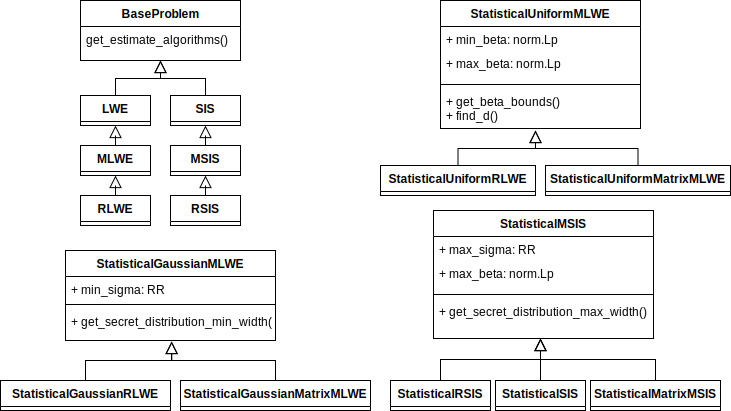
\includegraphics[width=1\textwidth]{graphics/problem_classes.pdf}
    \caption{Problem classes}\label{fig:problem-classes}
\end{figure}

$\texttt{LWE}$ and $\texttt{SIS}$ inherit from the base class $\texttt{BaseProblem}$ respectively. All instances provide a method $\texttt{get\_estimate\_algorithms()}$ that returns a list of algorithm instances that can be executed by the function $\texttt{estimate()}$. Furthermore, any instance of $\texttt{BaseProblem}$ can be compared to a bit security level (for more details, we refer the reader to the documentation). The $\texttt{LWE}$ class is initialized by the secret dimension $n$, a modulus $q$, the number of samples $m$, a $\texttt{secret\_distribution}$ and a $\texttt{error\_distribution}$. Both $\texttt{secret\_distribution}$ and $\texttt{error\_distribution}$ must be instances of the class $\texttt{distributions.Distribution}$. Instead of $\texttt{secret\_distribution}$ and $\texttt{error\_distribution}$, a bound of type $\texttt{norm.BaseNorm}$ must be set for $\texttt{SIS}$. Note that both {distributions.Uniform} and {distributions.Gaussian} are instances of $\texttt{norm.BaseNorm}$ and can thus be used as a bound. We compute the bound for a given distribution instance as described in \cref{sec:supported-distributions}.

For ring and module variants $\texttt{RLWE}$, $\texttt{RSIS}$ and $\texttt{MLWE}$, $\texttt{MSIS}$ respectively $n$ denotes the degree of the polynomial of the underlying ring $\mathcal{R}_q$. The module variants $\texttt{MLWE}$ and $\texttt{MSIS}$ take an addition parameter $d$ for the rank of the module.

While there exist special cases where the ring structure of problem instances can be exploited in an attack on LWE or SIS, % TODO: find examples
in general, the hardness of ring and Module variants is estimated by interpreting the coefficients of elements of $\mathcal{R}_q$ as vectors in $\mathbb{Z}_q^n$ \cite{ACDDPPVW18}. If we take into account the considerations we presented in \cref{sec:ring-module}, we can thus reduce ring and Module instances as follows when calling $\texttt{get\_estimate\_algorithms()}$ on the ring and module variant of $\texttt{LWE}$ and $\texttt{SIS}$:
\begin{itemize}
    \item RLWE$_{n, q, m, \chi} \longrightarrow$ LWE$_{n, q, m \cdot n, \chi}$
    \item MLWE$_{n, d, q, m, \chi} \longrightarrow$ LWE$_{n \cdot d, q, m \cdot n, \chi}$
    \item RSIS$_{n, q, m, \beta} \longrightarrow$ SIS$_{n, q, m \cdot n, \beta}$
    \item MSIS$_{n, d, q, m, \beta} \longrightarrow$ SIS$_{n \cdot d, q, m \cdot n, \beta}$
\end{itemize}


In addition to the base problem variants, we define some statistically secure variants for both LWE and SIS since some schemes depend on the unconditional hardness of either LWE or SIS. More precicely, we ask for parameters such an arbitrary powerful attacker can only break the scheme with probability less than $2^{-\texttt{sec}}$.

\paragraph{$\texttt{StatisticalGaussianMLWE}$.} For LWE, we define a statistically secure variant over a Gaussian distribution and over a uniform distribution. $\texttt{StatisticalGaussianMLWE}$ follows Corollary 7.5 and Theorem 7.4 in \cite{LPR13}. The mapping of the parameters in \cite{LPR13} to the usage in this work can be found in \cref{tab:mapping-LPR13}. We obtain the following theorem:

\begin{theorem}[Statistically Secure MLWE Over a Gaussian Distribution \cite{LPR13}]
    Let $\mathcal{R}$ be the ring of integers in the $m'$th cyclotomic number field $K$ of degree $n$, and $q \geq 2$ an integer.
    For positive integers $m \leq m + d \leq \text{poly}(n)$, let $\mathbf{A} = [ \mathbf{I}_{[m]} \mid \bar{\mathbf{A}}] \in (\mathcal{R}_q)^{[m] \times [m+d]}$, where $\mathbf{I}_{[m]} \in (\mathcal{R}_q)^{[m] \times [m]}$ is the identity matrix and $\bar{\mathbf{A}} \in (\mathcal{R}_q)^{[m] \times [d]}$ is uniformly random.
    Then with probability $1 - 2^{-\Omega(n)}$ over the choice of $\bar{\mathbf{A}}$, the distribution of $\mathbf{A}\mathbf{x} \in (\mathcal{R}_q)^{[m]}$ where each coordinate of $\mathbf{x} \in (\mathcal{R}_q)^{[m+d]}$ is chosen from a discrete Gaussian distribution of parameter $s > 2n \cdot q^{m / (m+d) + 2/(n (m+d))}$ over $\mathcal{R}$, satisfies that the probability of each of the $q^{n m}$ possible outcomes is in the interval $(1 \pm 2^{-\Omega(n)}) q^{-n }$ (and in particular is within statistical distance $2^{-\Omega(n)}$ of the uniform distribution over $(\mathcal{R}_q)^{[m]}$). % TODO change [x]times[y] notation???
\end{theorem}
% TODO: anything more? can you provide an intuition?

If a security parameter is passed and $\texttt{sec} > n$, we raise an exepction.
The resulting minimal standard deviation is stored in the instance variable $\texttt{min\_sigma}$ and the corresponding distribution can be obtained by calling $\texttt{get\_secret\_distribution\_min\_width()}$ on the class instance.



\paragraph{$\texttt{StatisticalUniformMLWE}$.} The authors of \cite{BDLOP18} describe statistically secure MLWE instances over a Uniform distribution with invertible elements. The samples $(\mathbf{A}', h_{\mathbf{A}'}(y))$ of the resulting MLWE instance are within statistical distance $2^{-\texttt{sec}}$ of $(\mathbf{A}', \mathbf{u})$ for uniformly distributed $\mathbf{u}$. % TODO: check formulation

We obtain the following theorem (for a mapping of the parameters, see \cref{tab:mapping-BDLOP18}): %TODO 

\begin{theorem}[Statistically Secure MLWE Over a Uniform Distribution \cite{BDLOP18}]
    Let $1 < d_2 < n$ be a power of 2. If $q$ is a prime congruent to $2d_2 + 1 \;(\text{mod } 4d_2)$ and
    \begin{equation}
        q^{m/(m+d)} \cdot 2^{2 \texttt{sec}/((m+d)\cdot n)} \leq 2 \beta < \frac{1}{\sqrt{d_2}} \cdot q^{1/d_2}
    \end{equation}
    then any (all-powerful) algorithm $\mathcal{A}$ has advantage at most $2^{-\texttt{sec}}$ in solving $\text{DKS}_{m,m+d,\beta}^\infty$, where $\text{DKS}^\infty$ is the decisional knapsack problem in $\ell_\infty$-norm.
\end{theorem}


Hence, we have:
\begin{align}
    \beta_{min} & = \frac{q^{m/(m+d)} \cdot 2^{2 \texttt{sec}/((m+d)\cdot n)}}{2} \\
    \beta_{max} & = \frac{1}{2\sqrt{d_2}} \cdot q^{1/d_2} - 1
\end{align}
% TODO: explain how to arrive at 2*\texttt{sec} instead of 256, für generellen \texttt{sec} parameter ...
% proof zum Beispiel im Anhang ...

The variable $d_2$ can be passed as an argument. If it is not passed, we try to find $d_2$ by iterating over all powers of $2$ that are smaller than $n$.
The resulting bounds are converted to $\ell_\infty$ and stored in the instance variables $\texttt{min\_beta}$ and $\texttt{max\_beta}$. We also provide an instance method $\texttt{get\_beta\_bounds()}$ to obtain a tuple of both.

For both statistically secure MLWE variants, we include the corresponding ring versions $\texttt{StatisticalGaussianRLWE}$ and $\texttt{StatisticalUniformRLWE}$ for $d=1$ and matrix versions $\texttt{StatisticalGaussianMatrixMLWE}$ and $\texttt{StatisticalUniformMatrixMLWE}$ for which the width and height of the matrix $\mathbf{A}$ in \cite{LPR13} can be passed instead of $m$ and $d$. % TODO: include instead of included?
% TODO: explain why this doesn't work for LWE


\paragraph{$\texttt{StatisticalMSIS}$.} We can find parameters for a statistically secure MSIS instance by following Section 4.1 of \cite{DOTT21}. The mapping of the parameters in \cite{DOTT21} is shown in \cref{tab:mapping-DOTT21}. More specifically, we ask to find a MLWE instance where the probability that non zero elements $\mathbf{r}$ in the Euclidean ball $B_{m}(0, 2B)$ satisfy $\hat{\mathbf{A}}_1 \cdot \mathbf{r} = \mathbf{0}$ is smaller than $2^{-\texttt{sec}}$. % TODO check that this is not a quote

The number of elements in $B_{m+d}(0, 2B)$ can be estimated from above as $|B_{m+d}(0, 2B)| \ll (2 \pi e /((m+d) n))^{(m+d) n/2} \cdot (2 B)^{(m+d) n}$. The scheme is statistically binding if the probability that non zero elements in $B_{m+d}(0, 2B)$ of radius $2B$ in $\mathcal{R}_q^{m+d}$ map to $\mathbf{0}$ in $\mathcal{R}_q^{m}$ is negligible. Hence, it must hold that $|B_{m+d}(0, 2B)|/q^{m n} \leq 2^{-\texttt{sec}}$ and we get:

% TODO: look for bound of ball without o(...) if change also change in docstring, check out wikipedia => heuristic. maybe find version not heuristic?
% add that this is approximation, see https://en.wikipedia.org/wiki/Volume_of_an_n-ball
% for small n?

\begin{align}
    \left(\sqrt{\frac{2 \pi e}{(m+d) \cdot n}} \cdot 2 B\right)^{(m+d) \cdot n} & \leq 2^{-\texttt{sec}} \cdot q^{m\cdot n}                                                                       \\
    B                                                                           & \leq 2^{\frac{-\texttt{sec}}{(m+d)\cdot n} - 1} \cdot q^\frac{m}{m+d} \cdot \sqrt{\frac{(m+d)\cdot n}{2 \pi e}}
\end{align}

We convert the bound $B$ to a Gaussian over $\ell_2$-norm by following the procedure described in \cref{sec:norm-bounds}: % TODO: add appropriate reference

\begin{equation}
    s  \approx x \sqrt{\frac{\pi}{(\texttt{sec} + 1) \ln(2)}}
\end{equation}

% TODO: rephrase to obtain a lemma?
The resulting parameters $B$ and $s$ can be accessed by the instance variables $\texttt{max\_sigma}$ and $\texttt{max\_beta}$ or by calling $\texttt{get\_secret\_distribution\_max\_width()}$ on the class instance.

As for statistically secure MLWE we again include a matrix version $\texttt{StatisticalMatrixMSIS}$ and a ring $\texttt{StatisticalRSIS}$ by setting $d=1$. In addition, the proof also applies to the base SIS variant and hence we include $\texttt{StatisticalSIS}$. Here the height of the matrix $n$ becomes the rank of the modulus in the MSIS instance, i.e. $d=n$, and the degree of the polynomial is $1$.




\section{Parameter Search and Configuration Options}
We now describe the main parameter search and estimate configuration options in our tool. The configuration can be customized by using the class $\texttt{algorithms.Configuration}$ and passed as an optional argument of $\texttt{param\_search.generic\_search()}$. It is also possible to directly estimate the cost of a list of parameter problems by calling the function $\texttt{problem.estimate()}$. For more details we again refer to the documentation.

\paragraph{Cost Models.} Attacks that use BKZ for lattice reduction require a cost model to estimate the number of CPU cycles in the SVP subroutine. Default cost models are shown in \cref{tab:costmodels}. We distinguish between estimates for classical, quantum, sieving and enumeration and each of these categories can be deselected by setting the respective parameter to $\texttt{False}$. At least one of classical and quantum and of sieving and enumeration respectively must be selected to make use of the default cost models.

Note that classical and quantum cost models cannot be directly compared with each other. The number of operations per second that can be executed by a quantum computer may be significantly smaller than for classical computers. % TODO add more?

If all are unselected custom cost models must be specified and passed as an argument. We included an option of taking the most conservative estimate for each category combination for a more efficient parameter search or estimation. Furthermore, we assigned a priority value on an ordinal scale to each cost model which enables us to first run cost models that yield a lower cost and thus terminate the estimation process earlier for an insecure parameter set. The priority values of the default cost models are derived from \cref{fig:costmodels}.
\begin{figure}[h]
    \centering
    \includegraphics[width=0.7\textwidth]{graphics/cost_models.png}
    \caption{Cost models}\label{fig:costmodels}
\end{figure}
The number of BKZ rounds can be configured by passing a function with parameters $\texttt{beta, d}$ where $\texttt{beta}$ is the block size and $\texttt{d}$ the lattice dimension. In the default configuration we use the more conservative Core-SVP model $\texttt{algorithms.BKZ\_SVP\_repeat\_core}$ \cite{ADPS16} in which the polynomial factor of the runtime complexity of BKZ is completely ignored. In addition, we provide a more realistic model $\texttt{algorithms.BKZ\_SVP\_repeat\_8d}$ for a BKZ cost of $8 \cdot d \cdot t_k$ BKZ rounds where $d$ again referes to the lattice dimension and $t_k$ is the number of clock cycles required for the SVP subroutine (see \cref{sec:bkz-8d}). % TODO maybe add a little more of evaluation here


\subsection{Generic Search and Estimate Algorithms}
The main functionality of our tool is encapsulated in the function $\texttt{param\_search.generic\_search()}$. The high-level idea of the search is presented in \cref{alg:generic-search}. We begin with an initial parameter set. We then create a list of problem instances generated by a $\texttt{parameter\_problem}$ function and estimate the cost of all instances in the list. If the list contains multiple SIS instances or multiple LWE instances, we attempt to reduce the instances to the easiest problem instance respectively. % TODO: include how, \cref{sec:problem-reduction} 
Once the $\texttt{estimate}$ function finds an instance that is insecure (i.e. the estimated attack cost in clock cycles is smaller than $2^{\texttt{sec}}$), it terminates the estimation procedure and returns an insecure result. We then use the $\texttt{next\_parameters}$ function to generate a list L of (multiple) new parameter sets from our current parameter set and sort each of the new parameter sets into an ordered list (duplicates are not accepted). The order is defined by a $\texttt{parameter\_cost}$ function. In the next step we retrieve the parameter set with the lowest cost from L and repeat the procedure until the cost estimation step returns a secure result. The result includes the estimates for all cost models and algorithms.

\begin{algorithm2e} % TODO: check if block is not of dimension kxk
    \SetKwBlock{Begin}{function}{end function}
    \Begin(generic\_search(sec, initial\_params, next\_parameters, parameter\_cost,  problem\_instance)) % TODO nxn???
    {
        L = OrderedList(initial\_params)\\
        \While{L $\neq \emptyset$}{
            current\_params = L.pop() \\
            instances = parameter\_problem(current\_params) \\
            result = estimate(instances, sec) \\
            \If{result is secure}{
                Return result\\
            }
            \Else{
                next\_param\_sets = next\_parameters(current\_params)\\
                \ForAll{param\_set in next\_param\_sets}{
                    sort param\_set into L according to parameter\_cost function\\
                }
            }
        }

    }
    \caption{Generic search} \label{alg:generic-search}
\end{algorithm2e}

The $\texttt{estimate}$ function can be configured to run in parallel in the configuration which may speed up the search, in particular if many cost models need to be tested (e.g. with configuration setting $\texttt{conservative=False}$ and long running algorithms like $\texttt{ARORA\_GB}$, $\texttt{CODED\_BKW}$ and $\texttt{PRIMAL\_DECODE}$ are used. The list of used algorithms can be changed in the configuration. We recommend to include $\texttt{PRIMAL\_USVP}$ for LWE instances and $\texttt{LATTICE\_REDUCTION}$ for SIS instances to make full use of early termination since the estimate algorithms for these attacks have a short runtime and yield relatively low cost estimates.


\cref{fig:SIS-algs}, \ref{fig:LWE-algs-small} and \ref{fig:LWE-algs-large} show the plots of runtime and performance tests for the various algorithms that can be used in our tool. In accordance with the results, we assigned priority values on an ordinal scale to the estimation algorithms. In \cref{tab:lwe-alg-prio} and \ref{tab:sis-alg-prio} we present the list of algorithms and their corresponding priority values and justify our choice. Algorithms with a smaller priority are expected to yield relatively good results quickly and can therefore be executed first. If the estimate result does not satisfy the specified security requirement we can terminate the estimation process early in order to maximize the efficiency of our search. Note that directly comparing the results for different algorithms, while convenient, is not always admissible as the compared algorithms may rely on different assumptions. Some algorithms may compute a more realistic cost while others may return a more conservative or even paranoid cost estimate (e.g. BKZ is used with the Core-SVP paranoid lower bound). The results have to be weighted carefully in order to guarantee the security of a given scheme in the forseable future while trying to keep the cost of using the scheme as low as possible. % TODO maybe move to conclusion...

\begin{figure}[]
    \centering
    \includegraphics[width=0.8\textwidth]{graphics/SIS_stddev=2,828_plots_1s.png}
    \caption{SIS instance with $\sigma=2.828,\; m=n^2, \; 2^{2n} < q < 2^{2n+1}$}\label{fig:SIS-algs}
\end{figure}

\begin{figure}[]
    \centering
    \includegraphics[width=0.8\textwidth]{graphics/LWE_stddev=0,125_plots_200s.png}
    \caption{LWE instance with $\sigma=0.125,\; m=\infty, \; 2^{n} < q < 2^{n+1}$}\label{fig:LWE-algs-small}
\end{figure}

\begin{figure}[]
    \centering
    \includegraphics[width=0.8\textwidth]{graphics/LWE_stddev=2,828_plots_200s.png}
    \caption{LWE instance with $\sigma=2.828,\; m=\infty, \; 2^{n} < q < 2^{n+1}$}\label{fig:LWE-algs-large}
\end{figure}

% TODO: how does dual attack without LLL work???
\begin{table}
    \centering
    \begin{tabular}[]{lll}
        \toprule
        Algorithm                 & Priority & Justification                                       \\\hline
        Meet-in-the-Middle        & 5        & fastest, high cost estimate, as prefilter           \\
        Primal-uSVP               & 10       & fast, low cost estimatate estimates                 \\
        Dual Attack               & 20       & fast, often higher estimates than primal-usvp       \\
        Dual Attack (without LLL) & 30       & fast, often higher estimates than dual              \\
        Coded-BKW                 & 90       & slow, somtimes very low cost estimate               \\
                                  &          & (for small stddev), does not always yield results   \\
        Decoding Attack           & 100      & slow, often higher estimates than faster algorithms \\
        Arora-Ge                  & 200      & extremely slow, often higher estimates,             \\
                                  &          & does not always yield results                       \\
        \bottomrule
    \end{tabular}
    \caption{LWE estimate algorithm priorities}\label{tab:lwe-alg-prio}
    \vspace{1cm}
    \begin{tabular}[]{lll}
        \toprule
        Algorithm                     & Priority & Justification                            \\\hline
        Lattice Reduction \cite{MR09} & 5        & fastest, low cost estimates              \\
        Lattice Reduction \cite{RS10} & 7        & same results as lattice-reduction,       \\
                                      &          & not always applicable                    \\
        Combinatorial Attack          & 10       & fast, often slightly higher cost results \\
        \bottomrule
    \end{tabular}
    \caption{SIS estimate algorithm prioritie}\label{tab:sis-alg-prio}
\end{table}

% TODO first finish section on algorithms
% - include plots
% - write about pro/cons
% - maybe add section of cost comparison for the algorithms of the previous section



\chapter{Usage Examples}
\section{Two Problem Search}\label{sec:two-problem-search}
% TODO: based on \cite{BDLOP18}
two problems lwe sis, what they are, how to solve it by the tool
\section{TODO: find other schemes to apply}


\chapter{Conclusion}
% TODO
- short summary
- tool
- future work: add more algorithms, extension to specify own algorithms (already possible but not really conveniant), estimator may be adapted in near future => adapt tool
- other things not part of my work but interesting



\printbibliography

All links were last followed on October 1, 2021.

\appendix
\addcontentsline{toc}{chapter}{Appendix}
\chapter{Additional Math}
\section{Linear Codes} \label{sec:linear-code} % TODO maybe move to Coded BKW, maybe too much...
Let $\mathbb{F}_q^n$ be the $n$-dimensional vector space over the field $\mathbb{F}_q$. A $q$-ary linear code $\mathcal{C}$ or $[n, k]$-code \cite{VanLint12} is a $k$-dimensional linear subspace of $\mathbb{F}_q^n$ such that $\mathbf{0} \in \mathcal{C}$, $\mathbf{x} + \mathbf{y} \in \mathcal{C}$ for all $\mathbf{x}, \mathbf{y} \in \mathcal{C}$ and $\gamma \mathbf{x} \in \mathcal{C}$ for $\mathbf{x} \in \mathcal{C}, \gamma \in \mathbb{F}_q$. There are $q^k$ different codewords in $\mathcal{C}$.

Let $\mathcal{C}$ be a $q$-ary linear $[n, k]$-code. The lattice over $\mathcal{C}$ \cite{GJS15} is defined as
\begin{equation}
    \Lambda(\mathcal{C}) = \left\{ \mathbf{x} \in \mathbb{R}^n \mid \exists \mathbf{y} \in \mathcal{C} : \mathbf{x} = \mathbf{y} \mod q  \right\}.
\end{equation} % TODO check
Similarly, for a lattice $\Lambda(\mathbf{B})$ a lattice code $\mathcal{C}$ defined by $\Lambda(\mathbf{B})$ and a shaping region $\mathcal{V} \subset \mathbb{R}^n$ (e.g. the Voronoi region, see \cref{eq:voronoi-region}) is a subspace of $\mathbb{R}^n$ such that all codewords are lattice vectors in $\Lambda(\mathbf{B})$ within the region $\mathcal{V}$ \cite{SFS08}:
\begin{equation}
    \mathcal{C} = \left\{ x \in \Lambda(\mathbf{B}) \mid x \in \mathcal{V} \right\}.
\end{equation} % TODO check

\chapter{Proofs}
\section{Proof of Norm Inequalities}\label{sec:proof-norm}
Let $p, q \in \mathbb{N}$ with $1 \leq p \leq q \leq \infty$. Then the following inequation holds:
\begin{align}
    \lim_{q' \rightarrow q}\| f \|_p & \leq \lim_{q' \rightarrow q} n^{\frac{1}{p} - \frac{1}{q'}}\| f \|_{q'}.
\end{align}

\begin{proof}
    For $\mathbf{x}, \mathbf{y} \in \mathbb{R}^n$ and $\frac{1}{u} + \frac{1}{v} = 1$, Hölder's inequality states that
    \begin{align*}
        \sum_{k=1}^n |\mathbf{x}_k| |\mathbf{y}_k| & \leq \left(\sum_{k=1}^n |\mathbf{x}_k|^u\right)^{\frac{1}{u}} \left(\sum_{k=1}^n |\mathbf{y}_k|^v\right)^{\frac{1}{v}}              \\
                                                   & = \left(\sum_{k=1}^n |\mathbf{x}_k|^u\right)^{\frac{1}{u}} \left(\sum_{k=1}^n |\mathbf{y}_k|^{\frac{u}{u-1}}\right)^{1-\frac{1}{u}}
    \end{align*}
    Following \cite{norm-relations}, we set $|\mathbf{x}_i| = |\mathbf{z}_i|^p$, $\mathbf{y}_i = 1$ and $u = \frac{q}{p} > 1$ and get

    \begin{align*}
        \sum_{k=1}^n |\mathbf{z}_i|^p  = \sum_{k=1}^n |\mathbf{z}_i|^p |\mathbf{y} & \leq \left(\sum_{k=1}^n |\mathbf{z}_i|^{p \frac{q}{p}}\right)^{\frac{p}{q}} \left(\sum_{k=1}^n 1^\frac{q}{q-p}\right)^{1-\frac{p}{q}} \\
                                                                                   & \leq n^{1-\frac{p}{q}} \left(\sum_{k=1}^n  |\mathbf{z}_i|^q\right)^{\frac{p}{q}}
    \end{align*}
    We now apply the definition of the $\ell_p$-norm (see \cref{sec:norms}) and obtain
    \begin{align*}
        \|\mathbf{z}\|_p = \left(\sum_{k=1}^n |\mathbf{z}_i|^p\right)^{\frac{1}{p}} & \leq  \left(n^{1-\frac{p}{q}} \left(\sum_{k=1}^n  |\mathbf{z}_i|^q \right)^{\frac{p}{q}} \right)^{\frac{1}{p}} \\
                                                                                    & = n^{\frac{1}{p}-\frac{1}{q}}\left(\sum_{k=1}^n |\mathbf{z}_i|^q\right)^{\frac{1}{q}}                          \\
                                                                                    & = n^{\frac{1}{p}-\frac{1}{q}} \|\mathbf{z}\|_q
    \end{align*}
\end{proof}

\chapter{Tables}
\section{Mapping of Parameters in Referenced Papers}
\begin{table}
    \centering
    \begin{tabular}[h]{lll}
        \toprule
        Parameters in \cite{LPR13} & Noation here & Represents                    \\\hline
        $l$                        & $m+d$        & width of matrix $\mathbf{A}$  \\
        $k$                        & $m$          & height of matrix $\mathbf{A}$ \\
        \bottomrule
    \end{tabular}
    \caption{Parameter Mapping from \cite{LPR13}}\label{tab:mapping-LPR13}
    \vspace{1cm}
    \centering
    \begin{tabular}[h]{lll}
        \toprule
        Parameters in \cite{BDLOP18} & Noation Here & Represents                                         \\\hline
        $k$                          & $m+d$        & width of matrix $[ \mathbf{I}_n \; \mathbf{A}' ]$  \\
        $n$                          & $m$          & height of matrix $[ \mathbf{I}_n \; \mathbf{A}' ]$ \\
        $d$                          & $d_2$        & variable                                           \\
        $N$                          & $n$          & degree of Ring polynomial                          \\
        \bottomrule
    \end{tabular}
    \caption{Parameter Mapping from \cite{BDLOP18}}\label{tab:mapping-BDLOP18}
    \vspace{1cm}
    \centering
    \begin{tabular}[h]{lll}
        \toprule
        Parameters in \cite{DOTT21} & Noation Here & Represents                            \\\hline
        $m'$                        & $m+d$        & width of matrix $\hat{\mathbf{A}}_1$  \\
        $m$                         & $m$          & height of matrix $\hat{\mathbf{A}}_1$ \\
        $B$                         & $B$          & norm-bound of secret                  \\
        $s$                         & $s$          & Gaussian width (not stddev)           \\
        $N$                         & $n$          & degree of polynomial                  \\
        \bottomrule
    \end{tabular}
    \caption{Parameter Mapping from \cite{DOTT21}}\label{tab:mapping-DOTT21}
\end{table}


\pagestyle{empty}
\renewcommand*{\chapterpagestyle}{empty}
\Versicherung
\end{document}